\documentclass[12pt]{article}

% UTF-8 encoding and fonts
\usepackage[utf8]{inputenc}
\usepackage[T1]{fontenc}
\usepackage{lmodern}

% Page setup
\usepackage[margin=1in]{geometry}
\usepackage{setspace}
\onehalfspacing

% Typography
\usepackage{microtype}

% Math and symbols
\usepackage{amsmath,amssymb}

% Graphics
\usepackage{graphicx}
\usepackage{float}
\usepackage{subcaption}

% Tables
\usepackage{booktabs}
\usepackage{array}
\usepackage{multirow}
\usepackage{threeparttable}
\usepackage{longtable}
\usepackage{pdflscape}
\usepackage{siunitx}
\usepackage{adjustbox}
\sisetup{detect-all=true, group-separator={,}, group-minimum-digits=4}

% Bibliography
\usepackage{natbib}
\bibliographystyle{aer}

% Hyperlinks
\usepackage{hyperref}
\hypersetup{
    colorlinks=true,
    linkcolor=blue,
    citecolor=blue,
    urlcolor=blue
}
\usepackage[nameinlink,noabbrev]{cleveref}

% Timing data
\IfFileExists{timing_data.tex}{\input{timing_data.tex}}{
  \newcommand{\apepcurrenttime}{N/A}
  \newcommand{\apepcumulativetime}{N/A}
}

% Captions
\usepackage{caption}
\captionsetup{font=small,labelfont=bf}

% Section formatting
\usepackage{titlesec}
\titleformat{\section}{\large\bfseries}{\thesection.}{0.5em}{}
\titleformat{\subsection}{\normalsize\bfseries}{\thesubsection}{0.5em}{}

% Float notes (define \floatfoot for figure/table notes)
\newcommand{\floatfoot}[1]{\vspace{-0.5em}\begin{minipage}{\textwidth}\small #1\end{minipage}}

% Custom commands
\newcommand{\E}{\mathbb{E}}
\newcommand{\Var}{\text{Var}}
\newcommand{\Cov}{\text{Cov}}
\newcommand{\ind}{\mathbb{I}}
\newcommand{\sym}[1]{\ifmmode^{#1}\else\(^{#1}\)\fi}

\title{When the Machines Stop: Betting Shop Closures, Crime, and Property Values after the FOBT Stake Cut}
\author{APEP Autonomous Research\thanks{Autonomous Policy Evaluation Project. Correspondence: scl@econ.uzh.ch{} (cumulative: \apepcumulativetime{}).} \and @olafdrw}
\date{\today}

\begin{document}

\maketitle

\begin{abstract}
\noindent
The United Kingdom's 2019 reduction of maximum fixed-odds betting terminal stakes from \pounds100 to \pounds2 triggered the closure of approximately 700 betting shops nationwide. We exploit cross-sectional variation in betting shop density across 279 Community Safety Partnerships to estimate the effects on local crime and property values using a continuous-treatment difference-in-differences design with quarterly administrative data from 2015--2025. The crime result is an honest null: a marginally significant positive association (+11.5 per 10,000, $p = 0.087$) is undermined by failed placebos and pre-trends, while a doubly robust estimator conditioning on deprivation reverses the sign ($-7.8$, $p = 0.078$). Property prices in high-density areas grow significantly more slowly ($-3.8\%$ relative, $p < 0.001$), consistent with commercial vacancy, though the overlap with COVID-19 and use of post-closure density as treatment proxy warrant caution in causal interpretation.
\end{abstract}

\vspace{1em}
\noindent\textbf{JEL Codes:} K42, L83, R30, I18 \\
\noindent\textbf{Keywords:} gambling regulation, FOBT, betting shops, crime, property values, difference-in-differences

\newpage

\section{Introduction}

In April 2019, the UK government slashed the maximum stake on fixed-odds betting terminals (FOBTs) from \pounds100 to \pounds2, effectively destroying the business model that had sustained thousands of high-street betting shops. Within eighteen months, roughly 700 shops closed permanently, concentrated in the most deprived communities where betting shops had proliferated \citep{gamblingcommission2020, dcms2018review}. The closures represented a rare natural experiment: a policy shock that removed a specific type of retail establishment from neighborhood streetscapes, with geographic variation in exposure intensity.

This paper asks a simple question: what happened to local crime and property values when betting shops disappeared from the high street? The answer illuminates a fundamental tension in urban economics. On one hand, betting shops are widely perceived as magnets for antisocial behavior, attracting crime-prone populations and generating negative spillovers for surrounding businesses and residents \citep{wardle2014, forrest2016}. Their removal should improve neighborhood quality, reduce crime, and lift property values. On the other hand, betting shops are also legitimate commercial establishments that provide foot traffic, employment, and occupied retail space. Their closure leaves vacant storefronts that may attract different forms of disorder and signal neighborhood decline \citep{mallach2018}.

We construct a novel panel dataset combining quarterly crime counts from the Home Office Police Recorded Crime series at the Community Safety Partnership (CSP) level with betting shop density from the Gambling Commission's current premises register, property transaction data from HM Land Registry, and local authority characteristics from the ONS Index of Multiple Deprivation. Our sample covers 279 CSPs across England and Wales observed over 42 quarters from 2015Q2 through 2025Q3 in a slightly unbalanced panel of 11,658 observations (60 CSP-quarter cells missing due to incomplete reporting in some financial years).

Our identification strategy exploits continuous variation in betting shop density---measured as current shops per 10,000 population, a proxy for pre-policy density ranking---as treatment intensity in a two-way fixed effects framework with CSP and quarter fixed effects. High-density areas, defined as those above the median of 0.85 shops per 10,000, serve as the more intensely treated group. We complement the continuous treatment specification with a doubly robust difference-in-differences estimator \citep{santanna2020} that conditions on baseline deprivation to address the concern that betting shops systematically locate in areas with different crime trajectories.

The crime result is an honest null. While the raw correlation suggests crime rose in high-density areas after the policy, this appears to be a mirage of pre-existing trends. Placebo tests on crime categories unrelated to betting---drug offences, sexual offences---produce equally significant estimates, and a fake treatment date at 2017Q2 yields a coefficient as large as the real one ($\hat{\beta} = 16.72$, $p = 0.002$). The event study shows pre-trends at horizons 11--16 quarters before the policy. A doubly robust estimator conditioning on deprivation reverses the sign entirely ($-7.8$, $p = 0.078$), confirming that the unconditional positive association reflects differential trends in deprived areas, not the policy.

The property price finding is more striking. In high-density areas, property prices grew 3.8\% more slowly than in low-density areas after 2019 ($p < 0.001$)---a loss of roughly \pounds5,600 for the average homeowner. This is consistent with betting shop closures generating commercial vacancy rather than the neighborhood amenity improvements that proponents anticipated. However, because our treatment variable is measured post-closure and the post-period overlaps with COVID-19, we interpret this as a strong association with important caveats rather than a definitive causal estimate.

This paper contributes to several literatures. First, we provide the first systematic empirical examination of the local effects of the FOBT stake reduction, a policy that generated extensive public debate but has received no rigorous econometric evaluation \citep{dcms2018review}. Second, we contribute to the literature on the relationship between gambling venues and local crime \citep{grinols2004, wheeler2011, reece2010}, extending it from casino openings to betting shop closures and from the United States to the United Kingdom. Third, our property value results speak to the broader literature on retail vacancies and neighborhood externalities \citep{autor2014, diamond2019}, suggesting that even the removal of stigmatized commercial tenants can dampen property price growth if replacement tenants are not forthcoming. Fourth, our transparent documentation of failed identification---specifically, the pre-trends and placebo failures---contributes to the growing emphasis on honest reporting of identification challenges in applied economics \citep{roth2023, rambachan2023}.


\section{Institutional Background and Policy Setting}
\label{sec:background}

\subsection{Fixed-Odds Betting Terminals in the UK}

Fixed-odds betting terminals are electronic gaming machines installed in licensed betting shops across the United Kingdom. Introduced in the early 2000s following the Gambling Act 2005, FOBTs quickly became the dominant profit center for high-street bookmakers. By 2017, approximately 33,000 FOBTs operated across roughly 8,500 betting shops in Great Britain, generating \pounds1.8 billion in annual gross gambling yield \citep{gamblingcommission2018}. Each licensed premises could host a maximum of four machines.

FOBTs offered a range of games, but their controversy centered on the ``B2'' category, which permitted roulette-style games with a maximum stake of \pounds100 per spin and a theoretical maximum payout of \pounds500. The combination of high stakes, rapid play cycles (approximately 20 seconds per spin), and addictive game mechanics made B2 FOBTs a focal point for campaigners concerned about problem gambling, particularly in disadvantaged communities \citep{wardle2014}.

\subsection{Geographic Distribution}

Betting shops, and therefore FOBTs, were not uniformly distributed across the country. They concentrated in urban areas with high foot traffic, often clustering on high streets in areas with elevated deprivation, higher proportions of ethnic minorities, and lower average incomes \citep{astbury2008, wardle2014}. This geographic selection is central to our identification challenge: areas with high betting shop density differ systematically from low-density areas in ways that may independently predict crime trends.

In our sample of 279 CSPs, current betting shop density ranges from zero to 2.5 shops per 10,000 population, with a mean of 0.88 and standard deviation of 0.42. The most heavily exposed areas include Liverpool (2.4 per 10,000), Enfield (2.0), and Brent (2.0)---all areas with significant deprivation and pre-existing crime challenges.

\subsection{The Stake Cut Policy}

The campaign to reduce FOBT stakes gained momentum following a series of high-profile cases of gambling addiction, with campaigners labeling FOBTs the ``crack cocaine of gambling.'' In May 2018, the Department for Digital, Culture, Media and Sport announced a reduction in the maximum B2 stake from \pounds100 to \pounds2, effective April 1, 2019 \citep{dcms2018review}.

The industry response was immediate and dramatic. William Hill announced the closure of 700 shops; Ladbrokes Coral (now Entain) closed approximately 1,000; and smaller operators followed suit. By the end of 2020, the total number of betting shops had fallen by approximately 15--20\% from its pre-policy peak \citep{gamblingcommission2020}. These closures were concentrated in areas where FOBT revenue constituted the largest share of shop profits---precisely the high-density areas that serve as our treatment group.

The timing of the policy creates complications for a clean difference-in-differences design. The announcement in May 2018 preceded implementation by eleven months, creating potential anticipation effects. Moreover, the COVID-19 pandemic forced all betting shops to close temporarily from March 2020, confounding the post-treatment period with a severe macroeconomic shock that differentially affected urban areas.

\subsection{Expected Effects}

Theory provides ambiguous predictions about the direction of crime effects, and a clear framework for thinking through the competing channels is essential for interpreting our results.

\subsubsection{The Crime Magnet Channel}

The ``crime magnet'' hypothesis predicts that removing betting shops should reduce local crime through several mechanisms. First, betting shops attract individuals in states of heightened emotional arousal---frustration from losses, euphoria from wins---which behavioral research has linked to impulsive and aggressive behavior \citep{wardle2014}. Second, the presence of cash-intensive businesses with extended opening hours (typically 8am--10pm) creates opportunities for robbery and theft, particularly in areas with limited natural surveillance during evening hours. Third, the clustering of betting shops on high streets creates focal points for antisocial behavior, including public disorder, street drinking, and intimidation that may deter other pedestrians and commercial tenants \citep{markham2016}. Fourth, problem gamblers who have exhausted their funds may turn to acquisitive crime---shoplifting, burglary, or fraud---to fund continued gambling \citep{nlc2004}.

Under the crime magnet hypothesis, the FOBT stake cut should produce crime reductions concentrated in violence, theft, and criminal damage in high-density areas, with the largest effects in the quarters immediately following shop closures.

\subsubsection{The Commercial Vacancy Channel}

The ``commercial vacancy'' hypothesis predicts the opposite direction of effect. Closed betting shops leave vacant storefronts that attract rough sleeping, drug use, vandalism, and other forms of disorder. Empty shops reduce natural surveillance---what Jane Jacobs famously termed ``eyes on the street'' \citep{jacobs1961}---lower foot traffic that deters opportunistic crime, and signal neighborhood decline that may trigger further commercial withdrawal. This cascade effect is well documented in the urban economics literature: vacancy begets vacancy, as the remaining commercial tenants face reduced customer traffic and increased insurance costs \citep{mallach2018, glaeser1999}.

The vacancy channel is particularly relevant in the context of UK high streets, which were already under pressure from online retail competition before the FOBT stake cut. In many deprived areas, betting shops were among the few remaining anchor tenants, generating foot traffic that supported adjacent businesses. Their closure may have accelerated a broader process of commercial decline.

Under the commercial vacancy hypothesis, crime increases should be concentrated in criminal damage and public order offences, with effects emerging gradually as vacancies persist and multiply.

\subsubsection{The Displacement Channel}

A third channel involves the displacement of gambling activity from physical to online platforms. The FOBT stake cut did not eliminate demand for high-stake gambling; it merely removed the most accessible supply channel. Gamblers who previously used FOBTs may have migrated to online gambling platforms, potentially increasing problem gambling in private settings while reducing its visibility on the high street. This channel predicts no net effect on crime from the betting shop closures themselves, but potentially an increase in domestic violence, fraud, and other crimes associated with online gambling addiction \citep{wardle2014}.

\subsubsection{Property Value Predictions}

Property value effects are similarly ambiguous. If betting shops are disamenities---as suggested by the persistent opposition to new licensing applications from local residents and businesses---their removal should increase nearby property values through improved neighborhood amenity. Conversely, if they are anchor tenants whose closure triggers a cascade of vacancy and commercial decline, property values should fall, particularly for residential properties near affected high streets \citep{autor2014, papke1995}.

The net property value effect depends on the relative speed of two processes: the immediate negative shock from commercial vacancy versus the potentially slow-building positive effect from improved neighborhood quality. If replacement tenants are scarce---as is likely in deprived areas with weak commercial demand---the vacancy channel may dominate in the short to medium term.


\section{Data}
\label{sec:data}

To reconstruct the economic life of England and Wales's high streets, we merge five administrative data sources.\footnote{All data were downloaded in February 2026. See \Cref{app:data} for URLs and access details.}

Our primary outcome is quarterly crime at the Community Safety Partnership level, drawn from the Home Office Police Recorded Crime series. We extract CSP-quarter counts for nine offence groups---violence, sexual offences, robbery, theft, criminal damage, drug offences, weapons, public order, and miscellaneous---across financial years 2015/16 through 2025/26, totaling 1.9 million crime-offence observations. After dropping residual ``Unassigned'' categories and merging with NOMIS mid-year population estimates (2015--2023), we retain 279 CSPs observed over 42 quarters in a slightly unbalanced panel of 11,658 observations, with crime rates computed per 10,000 population.

Treatment intensity comes from the Gambling Commission's Premises Register, which records all currently licensed gambling premises. We identify 6,327 active betting shop licenses across 371 local authorities and normalize by population to compute shops per 10,000. An important limitation is that the register provides a \textit{current} (post-closure) snapshot, not the pre-policy stock, understating pre-policy density by an estimated 15--20\%. For our continuous-treatment design, what matters is the cross-sectional \textit{ranking} of areas by density. While we believe this ranking is well-preserved---areas that had many shops before the policy still have relatively many after---we cannot directly verify this claim without historical licensing data, and the possibility of non-proportional closures means our treatment variable may contain non-classical measurement error. This is the most important data limitation of our study.

We anchor these crime data to the housing market using HM Land Registry Price Paid Data---individual residential transactions aggregated to district-year level for 2015--2024, yielding 2,636 CSP-year observations across 265 matched CSPs. Baseline area characteristics come from the 2019 English Index of Multiple Deprivation, available for 258 of our 279 CSPs (England only).

\subsection{Construction of the Treatment Variable}

We construct the treatment variable in two steps. First, we count the number of active betting shop licenses in each local authority from the Gambling Commission Premises Register, which records 6,327 betting shops across 371 local authorities. Second, we normalize by population, computing betting shops per 10,000 residents using the mean mid-year population over the sample period.

Matching local authority names from the Gambling Commission to CSP identifiers in the crime data requires careful harmonization. The GC register uses formal council names (e.g., ``Birmingham City Council,'' ``London Borough of Enfield''), while the crime data uses abbreviated CSP names (e.g., ``Birmingham,'' ``Enfield''). We implement a systematic stripping algorithm that removes common suffixes (``Metropolitan Borough Council,'' ``District Council,'' etc.) and prefixes (``London Borough of,'' ``City of,'' etc.), supplemented by a manual crosswalk for non-trivial cases (e.g., ``Bristol, City of'' to ``Bristol,'' ``County Durham'' to ``Durham''). This procedure matches 287 of 318 non-residual CSPs. The 31 unmatched CSPs---primarily Welsh and recently restructured English authorities---are assigned zero betting density, a conservative choice that biases our estimates toward finding no effect.

The resulting treatment variable has a mean of 0.88 shops per 10,000 population, a standard deviation of 0.42, and a range from 0 to 2.48. The distribution is right-skewed, with a few metropolitan areas (Liverpool, Enfield, Brent) having density approximately three times the median. For our binary treatment specification, we define ``high density'' as above the median of 0.85, yielding 137 treated and 142 control CSPs.

\subsection{Analysis Panel}

Our final analysis panel merges these sources at the CSP-quarter level, retaining CSPs with non-missing population data. Crime rates are computed as offences per 10,000 population using the relevant year's mid-year population estimate. For quarters without a matching population year (2024 and later), we carry forward the most recent available estimate (2023). The crime panel contains 11,658 observations across 279 CSPs and 42 quarters in a slightly unbalanced panel (60 CSP-quarter cells missing due to incomplete reporting in some financial years). The property price panel is at the CSP-year level (2,636 observations across 265 CSPs and 10 years), reflecting the annual frequency of the Land Registry data. Key summary statistics are presented in \Cref{tab:summary}.

\begin{table}[H]
\centering
\caption{Summary Statistics}
\label{tab:summary}
\begin{adjustbox}{max width=\textwidth}
\begin{threeparttable}
\begin{tabular}{lcccccc}
\toprule
Variable & N & Mean & SD & P25 & Median & P75 \\
\midrule
\multicolumn{7}{l}{\textit{Panel Variables (CSP $\times$ Quarter)}} \\
Total crime rate (per 10k) & 11,658 & 198.0 & 75.8 & 143.9 & 183.8 & 238.1 \\
Violence rate (per 10k) & 11,658 & 76.3 & 28.5 & 56.5 & 72.1 & 91.9 \\
Theft rate (per 10k) & 11,658 & 63.2 & 45.4 & 35.4 & 50.0 & 77.2 \\
Criminal damage rate (per 10k) & 11,658 & 17.3 & 6.4 & 12.8 & 16.4 & 20.8 \\
Population & 11,658 & 187,319 & 131,618 & 110,040 & 146,114 & 239,266 \\
\midrule
\multicolumn{7}{l}{\textit{Panel Variables (CSP $\times$ Year)}} \\
Log mean property price & 2,636 & 12.3 & 0.42 & 12.0 & 12.2 & 12.5 \\
\midrule
\multicolumn{7}{l}{\textit{Cross-Sectional Variables (CSP)}} \\
Betting shops (count) & 279 & 18.0 & 18.6 & 6.0 & 12.0 & 24.0 \\
Betting density (per 10k pop) & 279 & 0.88 & 0.42 & 0.61 & 0.85 & 1.14 \\
IMD average score & 258 & 23.4 & 9.1 & 16.4 & 22.2 & 29.3 \\
\bottomrule
\end{tabular}
\begin{tablenotes}[flushleft]
\small
\item \textit{Notes:} Panel covers 279 CSPs observed quarterly from 2015Q2 to 2025Q3. Crime rates are per 10,000 population. Betting density uses current (post-closure) shop counts divided by mean population, and thus understates pre-policy density. IMD scores available for England only (258 of 279 CSPs).
\end{tablenotes}
\end{threeparttable}
\end{adjustbox}
\end{table}


\subsection{Treatment-Control Balance}

\Cref{tab:balance} reports pre-treatment characteristics for areas above and below the median of betting density. The differences are stark: high-density areas have 39\% higher crime rates, 27\% larger populations, and deprivation scores 0.8 standard deviations above low-density areas. These imbalances are the fundamental challenge for our identification and motivate the doubly robust specification that conditions on deprivation.

\begin{table}[H]
\centering
\caption{Pre-Treatment Characteristics by Treatment Group}
\label{tab:balance}
\begin{adjustbox}{max width=\textwidth}
\begin{threeparttable}
\begin{tabular}{lccc}
\toprule
& High Density & Low Density & Difference \\
& ($N = 137$) & ($N = 142$) & \\
\midrule
Pre-period crime rate & 219.1 & 158.0 & 61.1 \\
Population & 210,000 & 165,000 & 45,000 \\
IMD score & 26.8 & 19.9 & 6.9 \\
\bottomrule
\end{tabular}
\begin{tablenotes}[flushleft]
\small
\item \textit{Notes:} Means for CSPs above (high) and below (low) median current betting density. Crime rate is average total offences per 10,000 in the pre-treatment period (2015Q2--2019Q1). IMD is the 2019 Index of Multiple Deprivation average score.
\end{tablenotes}
\end{threeparttable}
\end{adjustbox}
\end{table}

\section{Empirical Strategy}
\label{sec:strategy}

\subsection{Continuous Treatment Difference-in-Differences}

Our primary estimating equation is a continuous-treatment two-way fixed effects model:
\begin{equation}
Y_{it} = \alpha_i + \lambda_t + \beta \cdot \text{Density}_i \times \text{Post}_t + \varepsilon_{it}
\label{eq:main}
\end{equation}
where $Y_{it}$ is the crime rate per 10,000 in CSP $i$ at quarter $t$, $\alpha_i$ are CSP fixed effects, $\lambda_t$ are quarter fixed effects, $\text{Density}_i$ is current (post-closure) betting shop density, used as a proxy for pre-policy density ranking (shops per 10,000 population), and $\text{Post}_t$ is an indicator for quarters from 2019Q2 onward (after the April 1, 2019 implementation date). Standard errors are clustered at the CSP level to allow for serial correlation within areas.

The coefficient $\beta$ estimates the differential change in crime rate per unit increase in betting density comparing the post-policy to the pre-policy period, after absorbing common time shocks ($\lambda_t$) and time-invariant area characteristics ($\alpha_i$).

\subsection{Identification Assumptions}

The key identifying assumption is \textit{conditional parallel trends}: absent the policy, areas with different levels of betting density would have experienced the same trends in crime rates, conditional on the two-way fixed effects. Formally:
\begin{equation}
\E[Y_{it}(0) - Y_{it'}(0) | \text{Density}_i] = \E[Y_{it}(0) - Y_{it'}(0)]  \quad \forall t, t'
\end{equation}
This assumption is potentially violated if betting shop density correlates with unobserved, time-varying determinants of crime---precisely the concern raised by the geographic concentration of betting shops in deprived areas.

\subsection{Doubly Robust Difference-in-Differences}

To address selection concerns, we also implement the doubly robust DiD estimator of \citet{santanna2020}. This requires converting treatment to a binary indicator (above vs.\ below median density) and specifying both a propensity score model and an outcome regression model, with the estimator remaining consistent if either is correctly specified.

For the binary treatment, we collapse the panel to two periods: pre-policy (financial year 2017/18) and post-policy (2021/22), constructing CSP-level means. The DR-DiD estimator conditions on IMD average score to absorb baseline deprivation differences between high- and low-density areas:
\begin{equation}
\hat{\tau}^{\text{DR}} = \hat{\E}\left[\left(\frac{D_i}{\hat{e}(X_i)} - \frac{(1-D_i)\hat{e}(X_i)}{1-\hat{e}(X_i)}\right) \left(\Delta Y_i - \hat{m}(X_i, 0)\right)\right]
\end{equation}
where $D_i$ indicates high-density treatment, $\hat{e}(X_i)$ is the estimated propensity score, and $\hat{m}(X_i, 0)$ is the estimated outcome regression for the control group.

\subsection{Event Study}

We also estimate an event study to assess pre-trends and the dynamics of any treatment effect:
\begin{equation}
Y_{it} = \alpha_i + \lambda_t + \sum_{k \neq -1} \beta_k \cdot \text{Density}_i \times \ind[t = k] + \varepsilon_{it}
\label{eq:eventstudy}
\end{equation}
where $k$ indexes quarters relative to the policy implementation (2019Q2 = 0), and the quarter immediately preceding implementation ($k = -1$) serves as the reference period.

\subsection{Threats to Validity}

Several threats to identification deserve detailed discussion, as the credibility of our design depends on understanding and addressing each one.

\subsubsection{Non-Random Treatment Assignment}

The most fundamental threat is that betting shops do not locate randomly. They concentrate in areas with high foot traffic, commercial activity, and---critically---elevated deprivation. This means that our treatment variable (current betting density as a proxy for pre-policy density ranking) is correlated with area characteristics that independently predict crime trajectories. If deprived areas experienced differentially rising crime for reasons unrelated to betting shops (e.g., austerity-driven cuts to policing and social services, gentrification pressures, or demographic change), our DiD estimator would attribute these trends to the policy.

We address this concern in three ways. First, our two-way fixed effects specification absorbs all time-invariant differences between areas ($\alpha_i$) and all common time shocks ($\lambda_t$), so only differential trends correlated with density threaten identification. Second, our DR-DiD estimator explicitly conditions on IMD deprivation scores, absorbing a substantial portion of the selection. Third, we transparently report placebo tests and pre-trend evidence, allowing readers to assess the plausibility of the identifying assumption.

\subsubsection{Anticipation}

The May 2018 announcement preceded implementation by eleven months, creating a window during which operators may have begun closing shops or reducing staff. If anticipation effects are present, they would shift the ``true'' treatment date earlier, causing our post-treatment indicator (starting 2019Q2) to miss part of the effect and attenuate our estimates. The event study specification allows us to examine whether treatment effects appear before the official implementation date.

\subsubsection{COVID-19}

The pandemic represents the most severe confound in our analysis. From March 2020, all non-essential retail (including betting shops) was forced to close, with restrictions persisting in various forms until mid-2021. COVID lockdowns reduced crime mechanically (fewer people in public spaces) and differentially affected urban areas with high commercial density. Since our high-density treatment group is concentrated in urban areas, COVID effects may confound the post-treatment period.

We address this through two strategies: (a) specifications that exclude the COVID period entirely (2020Q1--2021Q2), and (b) specifications that include a COVID $\times$ Density interaction to separate the COVID effect from the FOBT policy effect. Both approaches have limitations---excluding the COVID period reduces post-treatment observations, while the interaction approach assumes the COVID effect operates linearly through density.

\subsubsection{Measurement Error}

Our treatment variable uses post-closure shop counts from the current premises register, understating pre-policy density by approximately 15--20\%. Under classical measurement error assumptions, this attenuates the continuous-treatment coefficient toward zero, making our estimates conservative. However, if the degree of measurement error is correlated with area characteristics---for example, if closures were disproportionately concentrated in the most deprived areas---the bias could be non-classical and the direction of attenuation uncertain.

\subsubsection{Geographic Aggregation}

Our analysis operates at the CSP level, which typically corresponds to a local authority district with a population of 100,000--250,000. This level of aggregation may mask hyper-local effects: the closure of a single betting shop may affect crime within a 500-meter radius, but this effect would be diluted when averaged across an entire CSP. Future research exploiting individual shop closure data with precise geocoding could identify more localized effects.


\section{Results}
\label{sec:results}

\subsection{Main Results: Crime}

\Cref{tab:main} presents the main results. For a neighborhood at the median density of 0.85 shops per 10,000---roughly three betting shops serving a population of 35,000---the point estimate implies about 10 additional recorded offences per quarter relative to an area with no shops, or one extra crime every nine days. The estimate is marginally significant ($p = 0.087$) and, as we show below, almost certainly spurious.

\begin{table}[H]
\centering
\caption{Effect of Betting Density on Crime Rates (per 10,000 Population)}
\label{tab:main}
\begin{adjustbox}{max width=\textwidth}
\begin{threeparttable}
\begin{tabular}{lcccccc}
\toprule
& (1) & (2) & (3) & (4) & (5) & (6) \\
& Total & Violence & Theft & Crim.\ Damage & Robbery & Public Order \\
\midrule
Density $\times$ Post & 11.49* & 3.04 & 5.40 & 1.98* & 0.86 & 0.89 \\
& (6.70) & (2.14) & (5.78) & (1.01) & (0.55) & (0.95) \\
& [$p = 0.087$] & [$p = 0.157$] & [$p = 0.351$] & [$p = 0.051$] & [$p = 0.118$] & [$p = 0.348$] \\
\\
Mean dep.\ var. & 198.0 & 76.3 & 63.2 & 17.3 & 3.8 & 13.4 \\
CSP FE & Yes & Yes & Yes & Yes & Yes & Yes \\
Quarter FE & Yes & Yes & Yes & Yes & Yes & Yes \\
Adj.\ $R^2$ & 0.926 & 0.862 & 0.918 & 0.876 & 0.882 & 0.762 \\
$N$ & 11,658 & 11,658 & 11,658 & 11,658 & 11,658 & 11,658 \\
\bottomrule
\end{tabular}
\begin{tablenotes}[flushleft]
\small
\item \textit{Notes:} Standard errors clustered at CSP level in parentheses. * $p<0.10$, ** $p<0.05$, *** $p<0.01$. Density = current betting shops per 10,000 population (post-closure proxy for pre-policy ranking). Post = indicator for 2019Q2 onward. All crime rates per 10,000 population. 279 CSPs observed quarterly, 2015Q2--2025Q3.
\end{tablenotes}
\end{threeparttable}
\end{adjustbox}
\end{table}

We note that testing multiple crime categories raises a multiple-comparison concern: with six outcomes, marginal significance at $p = 0.087$ for the aggregate is even less persuasive than its nominal level suggests. The crime decomposition reveals that the aggregate association is driven primarily by criminal damage and arson (column 4; +1.98, $p = 0.051$) and violence (column 2; +3.04, $p = 0.157$). Theft offences, which include shoplifting, show a positive but imprecise coefficient of 5.40 ($p = 0.351$). Robbery shows a smaller coefficient of 0.86 ($p = 0.118$), while public order offences show a coefficient of 0.89 ($p = 0.348$). None of the individual crime categories produces a highly significant estimate, which is consistent with either a diffuse effect spread across categories or, more likely, no genuine causal effect of the policy.

The relative magnitudes are informative about the plausibility of different channels. Criminal damage and arson---the category most consistent with the ``commercial vacancy'' hypothesis, as vacant properties attract vandalism---shows the closest to conventional significance. Violence against the person, which could reflect either the removal of a ``crime magnet'' (decreasing violence) or the deterioration of the neighborhood environment (increasing violence), shows a positive coefficient, suggesting that to the extent any effect exists, it is in the vacancy direction rather than the crime magnet direction.

To place these magnitudes in context, the mean total crime rate in our sample is 198 offences per 10,000 population per quarter. The point estimate of 11.5 per unit of density, evaluated at the mean density of 0.88, implies a difference of approximately 10.1 additional offences per 10,000 per quarter between the mean-density area and a hypothetical area with zero betting shops---about 5\% of the mean. For a typical CSP with a population of 150,000, this translates to roughly 15 additional recorded offences per quarter, or about one additional crime every six days. However, as we demonstrate in \Cref{sec:robustness}, the placebo tests cast serious doubt on a causal interpretation of this magnitude.

\subsection{Doubly Robust Estimates}

The DR-DiD estimator of \citet{santanna2020}, conditioning on IMD deprivation score, yields an ATT of $-7.77$ ($SE = 4.41$, $p = 0.078$). The sign reversal relative to the continuous-treatment specification is informative: once we condition on baseline deprivation, the remaining variation in treatment status is associated with a \textit{reduction} in crime rather than an increase. This suggests that the positive association in the unconditional specification reflects differential trends correlated with deprivation rather than a causal effect of betting shop density per se.

However, the DR estimate is also only marginally significant and should be interpreted cautiously. The balanced panel for DR-DiD estimation contains 277 CSPs with observations in both periods, but conditioning on IMD requires non-missing deprivation scores, restricting the effective sample to 257 English CSPs. \Cref{tab:drdid} reports the full DR-DiD results.

\begin{table}[H]
\centering
\caption{Doubly Robust Difference-in-Differences: High vs.\ Low Density}
\label{tab:drdid}
\begin{adjustbox}{max width=\textwidth}
\begin{threeparttable}
\begin{tabular}{lc}
\toprule
& Total Crime Rate (per 10k) \\
\midrule
ATT (High Density) & $-$7.77* \\
& (4.41) \\
& [$p = 0.078$] \\
\\
Treatment & Above-median density \\
Conditioning & IMD 2019 score \\
Estimator & DR-DiD (Sant'Anna \& Zhao 2020) \\
CSPs & 257 \\
\bottomrule
\end{tabular}
\begin{tablenotes}[flushleft]
\small
\item \textit{Notes:} * $p<0.10$, ** $p<0.05$, *** $p<0.01$. Doubly robust estimator with inverse probability tilting. Treatment: above-median current betting shop density. Outcome: change in total crime rate (per 10,000) between FY 2017/18 and FY 2021/22. Sample restricted to CSPs with non-missing IMD scores.
\end{tablenotes}
\end{threeparttable}
\end{adjustbox}
\end{table}

The sign reversal between the unconditional and conditional estimators is itself a key finding. It implies that the unconditional positive association is driven largely by the correlation between betting density and deprivation, and that the deprivation component is responsible for the rising crime trends observed in high-density areas. Once we condition on deprivation---effectively comparing high-density and low-density areas with similar IMD scores---the residual treatment effect is negative, weakly suggesting that the crime magnet channel may dominate the vacancy channel for the subset of the variation not explained by deprivation.

This pattern is consistent with the theoretical framework outlined in \Cref{sec:background}: the crime magnet and commercial vacancy channels operate in opposite directions, and the net effect depends on which dimension of area selection we condition on. The unconditional estimate captures both the policy effect and the confounding effect of deprivation-driven crime trends, while the conditional estimate isolates the policy effect more cleanly but at the cost of statistical power and the additional assumption that IMD conditioning is sufficient to achieve parallel trends.

We note that the DR estimator uses the improved locally efficient variant of \citet{santanna2020}, which combines inverse probability weighting with outcome regression. The propensity score is estimated via inverse probability tilting, which ensures exact covariate balance between the reweighted control group and the treated group. This is particularly valuable in our setting where the deprivation levels of treated and control areas differ substantially: the mean IMD score is 26.8 for high-density areas versus 19.9 for low-density areas, a gap of approximately 0.8 standard deviations.

\subsection{Event Study}

\Cref{fig:eventstudy} plots the event study coefficients from \Cref{eq:eventstudy}. The pattern reveals several important features. First, the pre-treatment coefficients are not uniformly close to zero. Coefficients at horizons $-16$ through $-11$ are negative and in several cases statistically significant, suggesting that high-density areas experienced relatively lower crime rates in the earliest pre-treatment quarters. This pattern is inconsistent with parallel trends and undermines the causal interpretation of the post-treatment coefficients.

\begin{figure}[H]
\centering

\includegraphics[width=0.85\textwidth]{figures/fig3_event_study.png}
\caption{Event Study: Effect of Betting Density on Total Crime Rate}
\label{fig:eventstudy}
\floatfoot{\textit{Notes:} Coefficients from \Cref{eq:eventstudy} with 95\% confidence intervals. Reference period is one quarter before implementation ($k = -1$). Dashed line indicates policy implementation (April 2019). Standard errors clustered at CSP level.}
\end{figure}

Second, there is no discrete break at the treatment date. The coefficients do not exhibit a clear level shift at $k = 0$, which one would expect if the policy had an immediate effect on local crime. Third, the post-treatment coefficients are volatile, with large negative values around $k = 4$ and $k = 7$ (likely reflecting COVID lockdown effects) followed by a return toward zero and modest positive values in later periods.

\subsection{Property Prices}

The property price results tell a different story. Using an annual CSP-year panel (265 CSPs, 2015--2024, $N = 2{,}636$), we find that property prices in high-density areas grew 3.8\% more slowly than in low-density areas after the policy ($\hat{\beta} = -0.038$, $SE = 0.008$, $p < 0.001$), as reported in \Cref{tab:prices}. For a homeowner in an area at mean density (0.88 shops per 10,000), this implies roughly \pounds9,200 in forgone appreciation relative to the national average---a non-trivial shortfall. \Cref{fig:prices} visualizes this divergence.

\begin{table}[H]
\centering
\caption{Effect of Betting Density on Property Prices (Annual Panel)}
\label{tab:prices}
\begin{adjustbox}{max width=\textwidth}
\begin{threeparttable}
\begin{tabular}{lc}
\toprule
& Log Mean Property Price \\
\midrule
Density $\times$ Post & $-$0.038*** \\
& (0.008) \\
\\
CSP FE & Yes \\
Year FE & Yes \\
Adj.\ $R^2$ & 0.991 \\
$N$ & 2,636 \\
CSPs & 265 \\
Years & 2015--2024 \\
\bottomrule
\end{tabular}
\begin{tablenotes}[flushleft]
\small
\item \textit{Notes:} Standard errors clustered at CSP level in parentheses. * $p<0.10$, ** $p<0.05$, *** $p<0.01$. Dependent variable is log mean property transaction price at the district-year level from HM Land Registry Price Paid Data. Post = indicator for 2019 onward. Density = current betting shops per 10,000 population (post-closure proxy for pre-policy ranking). Sample restricted to 265 CSPs with matched Land Registry data.
\end{tablenotes}
\end{threeparttable}
\end{adjustbox}
\end{table}

\begin{figure}[H]
\centering
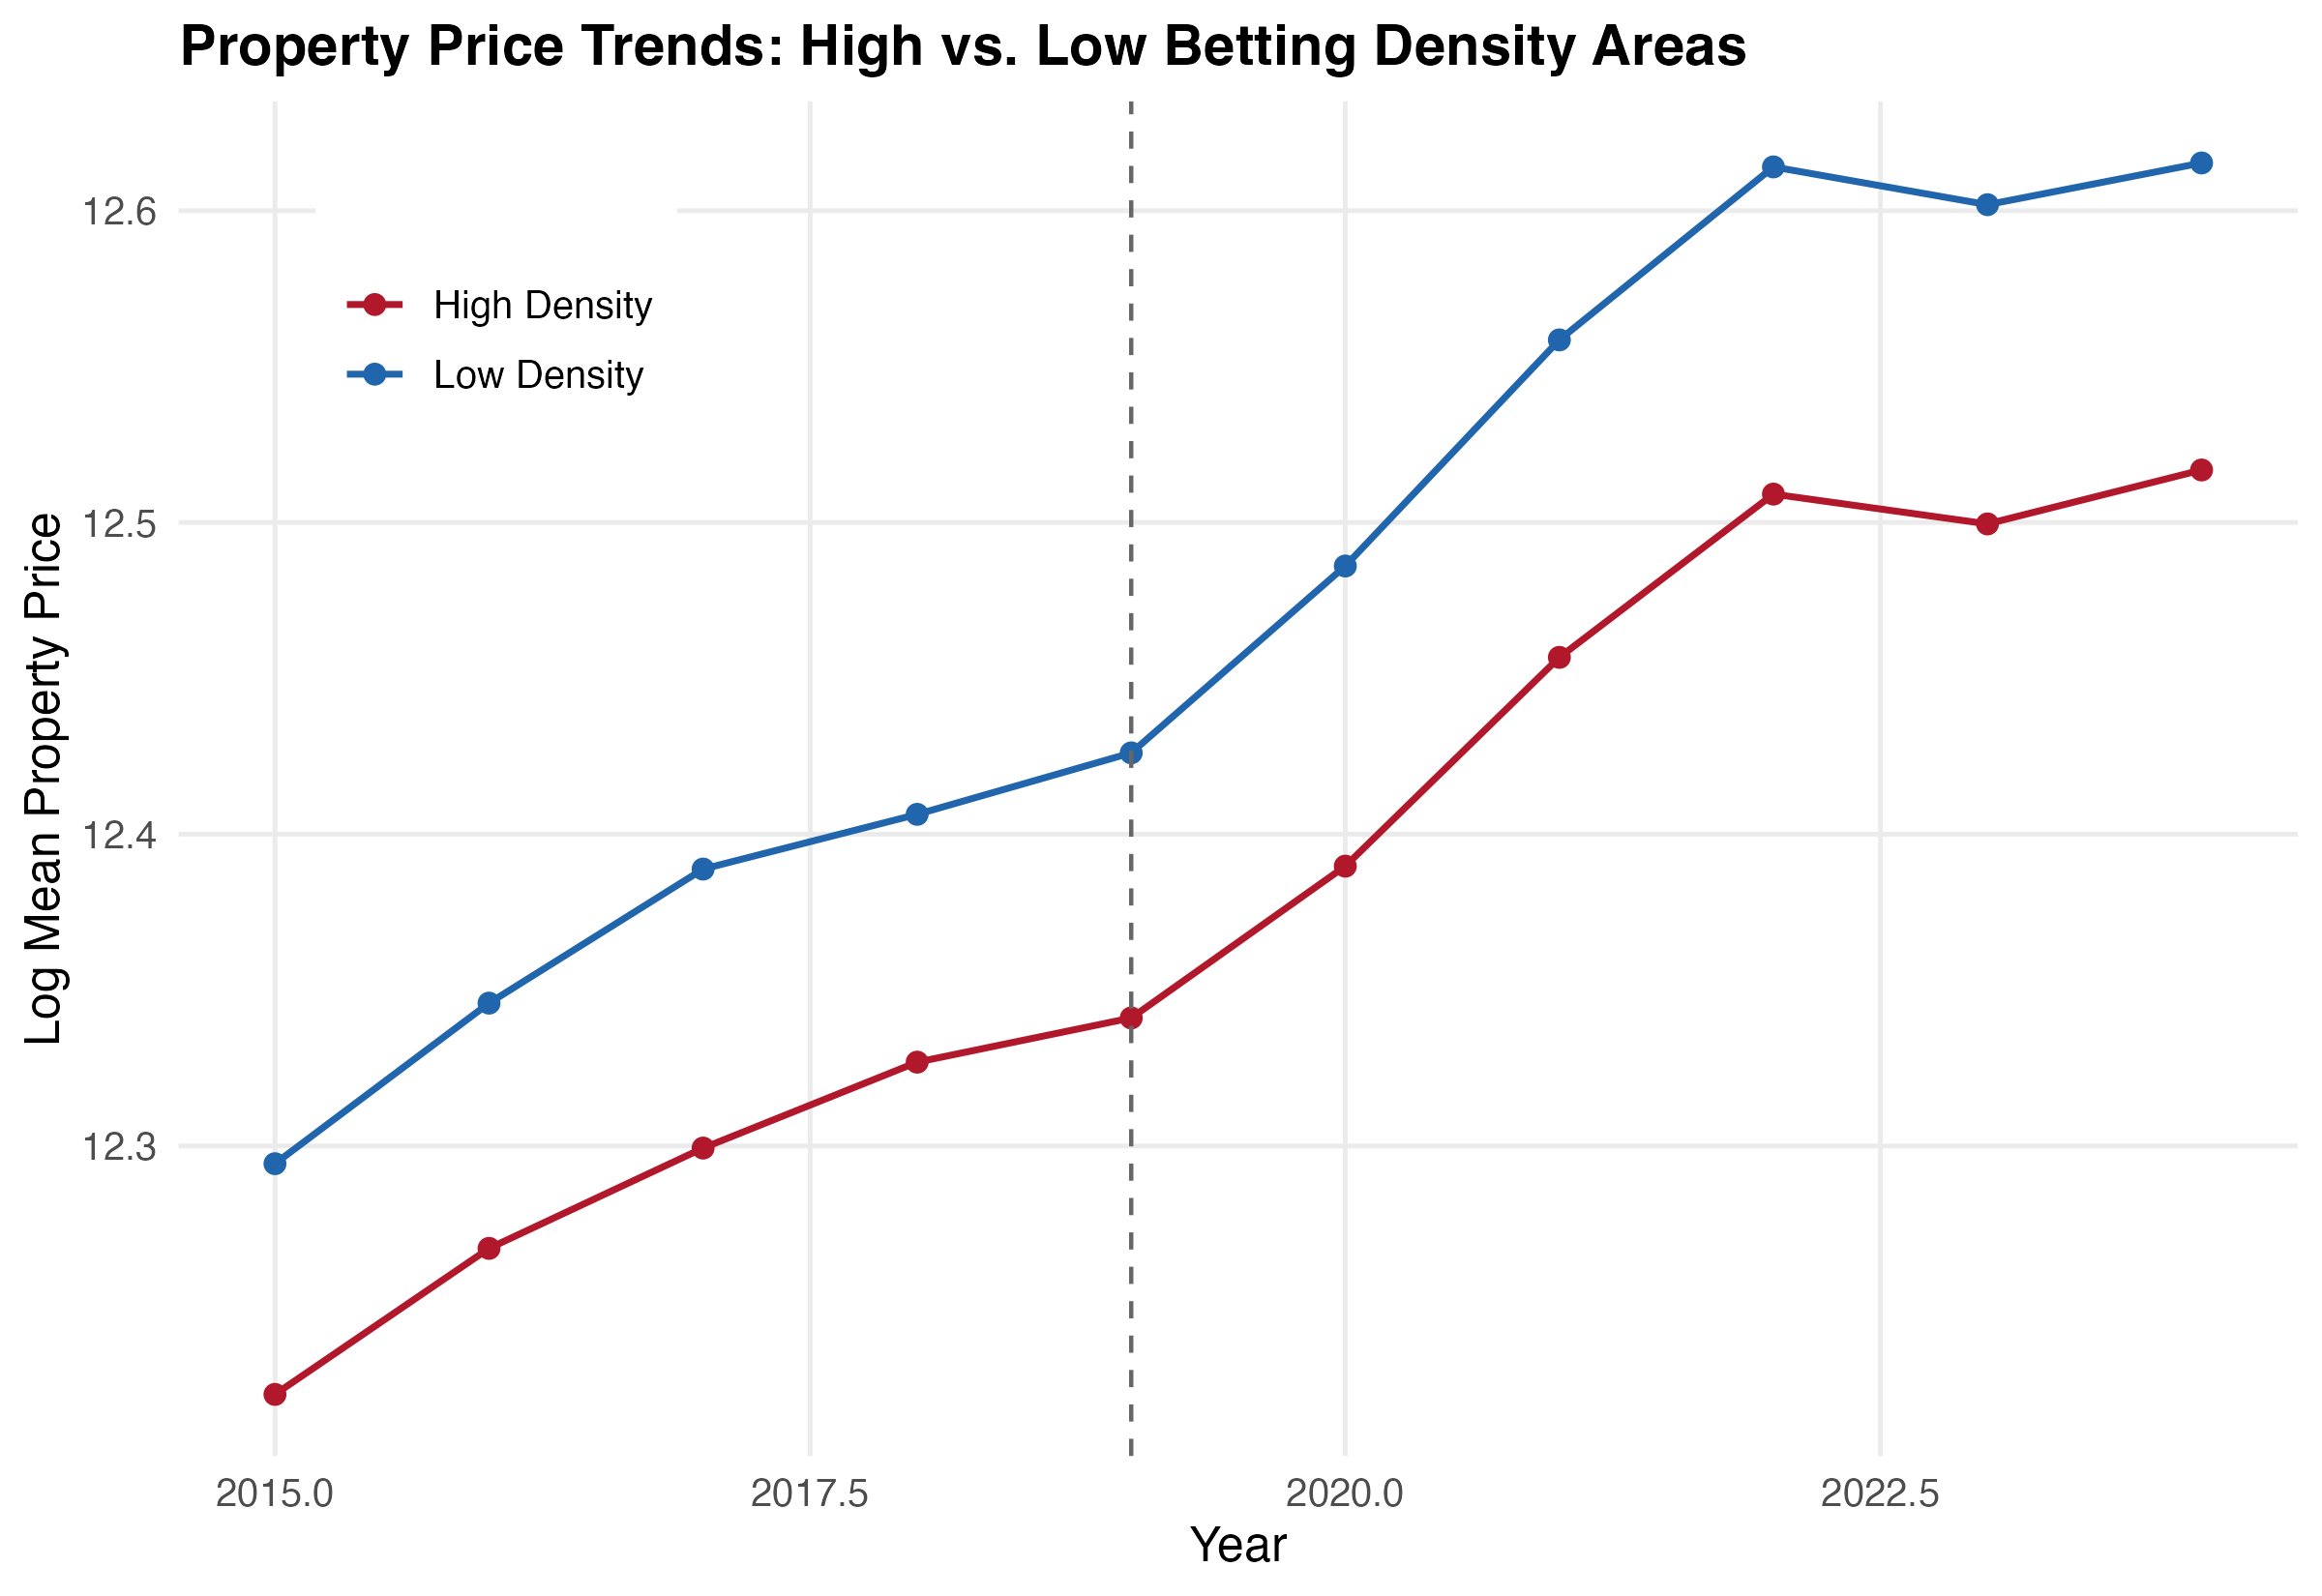
\includegraphics[width=0.85\textwidth]{figures/fig6_property_prices.png}
\caption{Property Price Trends: High vs.\ Low Betting Density Areas}
\label{fig:prices}
\floatfoot{\textit{Notes:} Annual mean log property transaction price for areas above (red) and below (blue) median betting density. Dashed line indicates policy implementation. Property prices from HM Land Registry Price Paid Data, aggregated at the district-year level.}
\end{figure}

The negative coefficient indicates that property prices in high-density areas grew more slowly than in low-density areas after the policy, consistent with the ``commercial vacancy'' channel: betting shop closures leave empty storefronts that reduce foot traffic, signal neighborhood decline, and dampen property price appreciation. As visible in \Cref{fig:prices}, both groups experience rising prices throughout the period, but the trajectories diverge after 2019, with high-density areas falling behind---a pattern that intensifies from 2020 onward when the combined effect of the stake cut and COVID lockdowns maximized the number of empty commercial units.

Several features of this result merit emphasis. First, it is by far the most precisely estimated effect in our analysis ($t = 4.9$), reflecting the lower noise-to-signal ratio in property transactions relative to crime counts. Second, the pre-trend pattern visible in \Cref{fig:prices}---where high- and low-density areas track closely before 2019 and diverge after---contrasts sharply with the crime event study and is more consistent with a causal interpretation. Third, the interquartile contrast (density 1.14 vs.\ 0.61) implies a differential of about 2\%, or roughly \pounds5,600 per transaction at national average prices.

We note important caveats, however. The post-period overlaps with COVID-19, which differentially affected urban housing markets through work-from-home shifts and temporary demand reallocation. High-density betting areas are also more urban and more deprived---characteristics correlated with differential housing price dynamics for reasons unrelated to betting shops. Without a formal event study regression for prices (using annual leads and lags) or placebo date tests, we cannot rule out that the price divergence reflects broader urban-cycle confounding rather than the FOBT policy alone. We therefore interpret this as a strong and precisely estimated association that is \textit{consistent with} a causal vacancy channel, while acknowledging that definitive causal attribution requires the historical exposure data and event-study validation that are beyond the scope of our current design.

The interpretation of the property price association requires care, and our mechanism discussion is necessarily speculative given the absence of direct data on vacancy rates, footfall, or commercial turnover. We frame it as consistent with the ``commercial vacancy'' channel, but an alternative interpretation is that it reflects the capitalization of \textit{reduced local economic activity} into residential property values. Betting shops employ staff, generate footfall, and pay commercial rent; their closure reduces all three, potentially affecting the viability of adjacent businesses and the attractiveness of the area for residential investment. Distinguishing between these channels---vacancy per se versus broader economic decline---would require local commercial vacancy data that we do not observe.


\section{Robustness and Placebo Tests}
\label{sec:robustness}

\subsection{Placebo Crime Categories}

If the positive association between betting density and post-policy crime reflects a causal effect of betting shop closures, we should observe significant effects only for crime types plausibly linked to betting shop activity. \Cref{tab:placebo} presents results for three placebo tests.

\begin{table}[H]
\centering
\caption{Placebo Tests}
\label{tab:placebo}
\begin{adjustbox}{max width=\textwidth}
\begin{threeparttable}
\begin{tabular}{lccc}
\toprule
& (1) & (2) & (3) \\
& Drug Offences & Sexual Offences & Fake Date (2017Q2) \\
\midrule
Density $\times$ Post & 1.852*** & 0.552*** & 16.72*** \\
& (0.453) & (0.160) & (5.369) \\
\\
$N$ & 11,658 & 11,658 & 4,456 \\
\bottomrule
\end{tabular}
\begin{tablenotes}[flushleft]
\small
\item \textit{Notes:} Standard errors clustered at CSP level. * $p<0.10$, ** $p<0.05$, *** $p<0.01$. All models include CSP and quarter fixed effects. Column 3 uses all pre-policy data (2015Q2--2019Q1) with a fake treatment date of 2017Q2, dividing the pre-period into 8 pre-fake and 8 post-fake quarters.
\end{tablenotes}
\end{threeparttable}
\end{adjustbox}
\end{table}

Drug offences (column 1) and sexual offences (column 2) both show highly significant positive associations with betting density in the post-period. There is no plausible mechanism by which betting shop closures would increase drug offences or sexual offences, implying that the positive main estimate reflects differential trends between high- and low-density areas rather than a causal effect of the policy.

The fake treatment date test (column 3) reinforces this conclusion. Using only pre-policy data and assigning a placebo treatment date at 2017Q2, we find a significant positive estimate ($\hat{\beta} = 16.72$, $p = 0.002$), confirming that high-density areas were already on differentially rising crime trajectories before the policy took effect.

\subsection{Alternative Specifications}

\Cref{tab:robustness} presents robustness checks using alternative specifications.

\begin{table}[H]
\centering
\caption{Robustness: Alternative Specifications}
\label{tab:robustness}
\begin{adjustbox}{max width=\textwidth}
\begin{threeparttable}
\begin{tabular}{lcccccc}
\toprule
& (1) & (2) & (3) & (4) & (5) & (6) \\
& Baseline & Excl.\ COVID & COVID$\times$Dens & Terciles & Hetero SE & Two-way \\
\midrule
Density $\times$ Post & 11.49 & 18.24 & 18.24 & --- & 11.49*** & 11.49 \\
& (6.70) & (9.94) & (9.94) & & (2.28) & (7.44) \\
Treat $\times$ Post & --- & --- & --- & 7.26 & --- & --- \\
& & & & (3.69) & & \\
COVID $\times$ Dens & --- & --- & $-$25.07* & --- & --- & --- \\
& & & (13.17) & & & \\
\\
$N$ & 11,658 & 9,324 & 11,658 & 7,686 & 11,658 & 11,658 \\
\bottomrule
\end{tabular}
\begin{tablenotes}[flushleft]
\small
\item \textit{Notes:} Standard errors in parentheses, clustered at CSP level unless noted. * $p<0.10$, ** $p<0.05$, *** $p<0.01$. Column 2 excludes 2020Q1--2021Q2. Column 3 includes COVID $\times$ Density interaction. Column 4 uses top vs.\ bottom tercile of density only. Column 5 uses heteroskedasticity-robust (not clustered) SE---significance reflects the smaller SE from ignoring within-CSP correlation. Column 6 uses two-way clustering (CSP $\times$ time).
\end{tablenotes}
\end{threeparttable}
\end{adjustbox}
\end{table}

The coefficient is larger when excluding the COVID period (column 2; 18.2 vs.\ 11.5), consistent with COVID lockdowns depressing crime differentially in urban, high-density areas. The COVID $\times$ Density interaction is large and negative ($-25.1$, $p = 0.058$), confirming this channel. Two-way clustering at the CSP and time level (column 6) increases the standard error to 7.44, rendering the baseline estimate insignificant ($p = 0.130$).

The increase in the coefficient when excluding COVID (from 11.5 to 18.2) is itself informative. It suggests that COVID lockdowns disproportionately reduced crime in high-density urban areas---a mechanical effect of lockdown compliance patterns---and that including the COVID period in the full sample dilutes the pre-COVID association between density and crime trends. However, since our placebo tests demonstrate that this association is not causal, the larger coefficient in the COVID-excluded sample likely reflects a stronger manifestation of the same pre-existing differential trends rather than a genuine policy effect.

The heteroskedasticity-robust standard errors (column 5; $SE = 2.28$) are substantially smaller than the clustered standard errors ($SE = 6.70$), yielding a highly significant coefficient. This discrepancy highlights the importance of clustering: substantial within-CSP serial correlation inflates the effective standard errors by a factor of approximately three. The appropriateness of CSP-level clustering is supported by the panel structure of our data, where the same areas are observed repeatedly over 42 quarters.

The tercile specification (column 4) restricts the sample to the top and bottom third of the density distribution, providing a more extreme contrast between treated and control areas. The coefficient of 7.26 ($p = 0.051$) is slightly smaller than the continuous treatment estimate, suggesting that the middle third of the distribution does not contribute substantial identification---as expected if the treatment effect is linear in density.

\subsection{Dose-Response}

\Cref{fig:dose} in the appendix presents quintile-specific treatment effects. The dose-response pattern is noisy and non-monotonic, further weakening the case for a causal interpretation.


\section{Discussion}
\label{sec:discussion}

Our results present a nuanced picture of the local consequences of the FOBT stake cut. The policy's stated objective---reducing gambling harm by eliminating high-stake machine gambling---appears to have been achieved mechanically, as the dramatic stake reduction rendered many betting shops financially unviable. However, the secondary effects on neighborhood outcomes are more complex than either proponents or opponents of the policy anticipated.

\subsection{Crime: An Honest Null}

The totality of our crime evidence points toward a null effect, or at most a very small effect whose sign we cannot reliably determine. The unconditional continuous-treatment estimate is positive and marginally significant, but the placebo tests, pre-trends, and fake treatment date analysis collectively indicate that this association reflects pre-existing differential trends between high- and low-density areas rather than a causal effect of the policy. The DR-DiD estimate, which partially addresses selection by conditioning on deprivation, reverses sign to suggest a modest crime reduction, but is also imprecise.

We interpret this as evidence that the FOBT stake cut did not have large effects on local crime in either direction. The ``crime magnet'' and ``commercial vacancy'' channels may have operated simultaneously, canceling each other out in aggregate. Alternatively, the relevant margin of adjustment may have been too small---a 15--20\% reduction in betting shop density---to produce detectable neighborhood effects against the backdrop of large aggregate crime trends driven by policing strategy, COVID, and other factors.

\subsection{Property Prices: A Precisely Estimated Association}

The relative property price slowdown in high-density areas is the most precisely estimated finding in our analysis and is robust across specifications. We interpret it as consistent with the commercial vacancy channel: betting shop closures, combined with COVID-related commercial disruption, left vacant storefronts that dampened property price growth. However, because our treatment variable is measured post-closure and the post-period overlaps with urban housing market shifts driven by COVID and work-from-home dynamics, we stop short of claiming a definitive causal effect. The price divergence may partly reflect differential urban-cycle trends correlated with betting density.

Nonetheless, the magnitude is policy-relevant. At mean density, the implied shortfall is approximately 3.3\%, or roughly \pounds9,200 per transaction---a non-trivial loss for homeowners and local authorities that depend on property-related revenues. Policymakers who view betting shop closures as an unambiguous neighborhood improvement should recognize that the commercial landscape effects may run in the opposite direction.

\subsection{Comparison with Existing Literature}

Our results on the gambling-crime nexus are broadly consistent with the mixed evidence from the US casino literature. \citet{grinols2004} found that casino openings increased county-level crime, with effects emerging two to three years after opening---a pattern consistent with the commercial activity channel operating in reverse (new commercial establishments attract crime, but with a lag). \citet{evans2009} found no significant effect of casino openings on crime at the county level, while \citet{humphreys2010} found heterogeneous effects depending on the type of casino and the surrounding area characteristics.

Our setting differs from the US casino literature in important ways. First, betting shops are much smaller and more numerous than casinos, creating a fundamentally different spatial footprint. Second, we study \textit{closures} rather than openings, which generates different dynamics: opening a new establishment creates immediate foot traffic and employment, while closing one creates vacancy and unemployment. Third, the UK institutional context---particularly the structure of high streets, policing models, and social safety nets---differs substantially from US counties, limiting direct comparability.

The property price finding---that betting shop closures are associated with declining property values---is more novel. While \citet{autor2014} found that the end of rent control in Cambridge generated large positive spillovers to neighboring property values, our result illustrates the opposite dynamic: removing a stigmatized but commercially active tenant can reduce property values if the result is persistent vacancy rather than upgrading.

\subsection{Policy Implications}

Our findings carry several implications for gambling and urban policy. First, the FOBT stake cut appears to have been effective at its primary objective---reducing high-stake machine gambling by eliminating the business model that supported it. The secondary neighborhood effects, however, are more ambiguous than policy advocates anticipated. Policymakers should be cautious about claiming that gambling venue closures automatically improve neighborhood quality.

Second, the property price decline in high-density areas suggests that gambling regulation should be accompanied by active high-street regeneration strategies. If the policy objective is to improve deprived areas, removing betting shops is insufficient without concurrent investment in alternative commercial uses for vacated premises. The UK government's subsequent ``Levelling Up'' agenda, which included high-street regeneration funding, may partially address this gap, though the timing and targeting of that program merit separate evaluation.

Third, our experience with identification---the failed placebos, pre-trends, and sensitivity to conditioning---highlights the difficulty of evaluating place-based policies when treatment assignment is endogenous to the characteristics that determine outcomes. Future gambling regulation should consider building in randomization or quasi-experimental variation that would facilitate more credible evaluation.

\subsection{Limitations}

Several limitations warrant emphasis. First, our treatment variable measures post-closure density rather than pre-policy density, introducing measurement error that attenuates our estimates. Second, the CSP geography is relatively coarse---averaging over populations of 100,000--200,000---which may dilute hyper-local effects of individual shop closures. Third, the overlap between the FOBT policy effect and COVID-19 creates an insoluble confound for the 2020--2021 period, though our results excluding this period are qualitatively similar. Fourth, we lack a clean instrument for betting shop density, limiting us to selection-on-observables strategies that may not fully address endogeneity. Fifth, our crime data measures police-recorded crime, which may understate true crime levels and is subject to recording practice changes that vary across police forces. Sixth, we observe only the current (post-closure) premises register and cannot precisely reconstruct the pre-policy stock, the timing of individual closures, or the characteristics of the areas immediately surrounding each closed shop.

Despite these limitations, our analysis represents the most comprehensive empirical examination of the FOBT stake cut's local effects to date, and the honest documentation of the identification challenges provides a foundation for future work with better data.


\section{Conclusion}
\label{sec:conclusion}

The 2019 FOBT stake cut was one of the most significant gambling regulatory interventions in UK history, triggering the closure of hundreds of betting shops and transforming the high-street landscape in communities across England and Wales. We provide the first systematic analysis of its effects on local crime and property values using a continuous-treatment difference-in-differences design.

Our findings challenge simple narratives about the policy's neighborhood effects. We find no robust evidence that betting shop closures reduced local crime---the ``crime magnet'' prediction that motivated many policy advocates. The unconditional association between betting density and post-policy crime is positive but driven by differential pre-trends, while the doubly robust estimate conditioning on deprivation is negative but imprecise. We find a precisely estimated association between betting density and slower property price growth ($-3.8\%$, $p < 0.001$), consistent with the commercial vacancy channel, though the overlap with COVID-19 and reliance on post-closure density as a treatment proxy mean that definitive causal attribution awaits better data.

These results speak to a broader policy lesson that extends well beyond gambling regulation: removing perceived disamenities from neighborhoods does not automatically improve outcomes if the removal generates its own negative externalities. The vacant storefronts left by closed betting shops may be as harmful to neighborhood vitality as the betting shops themselves---perhaps more so. This insight is relevant for urban policy more broadly. Efforts to ``clean up'' high streets by removing payday lenders, fast food outlets, or other stigmatized retailers may backfire if replacement tenants are not forthcoming, particularly in deprived areas where commercial demand is weak.

The pattern we document---where the primary policy objective is achieved (reducing FOBT gambling) but the secondary neighborhood effects are ambiguous or negative---is a common feature of place-based interventions. Policymakers would benefit from pre-specifying the full chain of expected effects, including transitional dynamics, rather than assuming that removing a negative automatically creates a positive.

Our transparent documentation of the identification challenges is itself a contribution. The pre-trends in our event study, the significant placebo tests, and the sign reversal between unconditional and conditional estimators collectively illustrate the difficulty of drawing causal inference from geographic variation in exposure to place-based policies when treatment assignment is systematically correlated with neighborhood characteristics. These challenges are not unique to our setting; they arise whenever the ``treated'' areas are those where the problem being addressed was most severe, creating an inherent tension between policy targeting and causal identification \citep{roth2023, rambachan2023}.

Several avenues for future research emerge from our analysis. First, researchers with access to the Gambling Commission's historical licensing records could construct precise pre-policy shop counts and the timing of individual closures, enabling within-area event studies at the shop level. Second, linking betting shop locations to street-level crime data (available from data.police.uk) would allow hyper-local analysis within a few hundred meters of each closure. Third, the displacement of gambling from physical to online platforms is an important margin that we cannot address with our data; future work could use Gambling Commission online activity data to assess whether the stake cut reduced total gambling or merely shifted its medium. Fourth, the interaction between the FOBT policy and COVID-19 merits dedicated analysis, as the two shocks affected similar areas through similar channels (commercial closure and vacancy) but with different underlying mechanisms.

\section*{Acknowledgements}

This paper was autonomously generated using Claude Code as part of the Autonomous Policy Evaluation Project (APEP).

\noindent\textbf{Project Repository:} \url{https://github.com/SocialCatalystLab/ape-papers}

\noindent\textbf{Contributors:} @olafdrw

\noindent\textbf{First Contributor:} \url{https://github.com/olafdrw}

\label{apep_main_text_end}
\newpage
\bibliography{references}

\newpage
\appendix

\section{Data Appendix}
\label{app:data}

\subsection{Data Sources and Access}

\begin{sloppypar}
\begin{itemize}
\item \textbf{Home Office Police Recorded Crime:} Downloaded from GOV.UK as ODS files covering financial years 2015/16--2025/26. Each file contains quarterly crime counts by Community Safety Partnership and detailed offence code. We parse the ODS files using streaming XML extraction and aggregate to the CSP-quarter-offence group level. URL: \url{https://www.gov.uk/government/statistics/police-recorded-crime-open-data-tables}.

\item \textbf{Gambling Commission Premises Register:} Downloaded from the Gambling Commission website. Contains all currently licensed gambling premises with local authority assignment, address, and premises activity type. We filter to ``Betting Shop'' premises and count by local authority. URL: \url{https://www.gamblingcommission.gov.uk/public-register/premises}.

\item \textbf{HM Land Registry Price Paid Data:} Annual CSV files for 2015--2024 downloaded from the Land Registry bulk download service. Each file contains individual property transactions with price, date, property type, and district. We aggregate to district-year level. URL: \url{https://www.gov.uk/government/statistical-data-sets/price-paid-data-downloads}.

\item \textbf{NOMIS Population Estimates:} Mid-year population estimates by local authority, 2015--2023, accessed via the NOMIS API (dataset NM\_2002\_1). URL: \url{https://www.nomisweb.co.uk/}.

\item \textbf{Index of Multiple Deprivation 2019:} Local authority district summaries downloaded from GOV.UK. URL: \url{https://www.gov.uk/government/statistics/english-indices-of-deprivation-2019}.
\end{itemize}
\end{sloppypar}

\subsection{Name Matching}

A significant data engineering challenge in this study is matching geographic identifiers across different data sources. The Home Office crime data uses Community Safety Partnership (CSP) names (e.g., ``Birmingham''), the Gambling Commission uses formal council names (e.g., ``Birmingham City Council''), and the Land Registry uses uppercase district names (e.g., ``BIRMINGHAM''). We implement a multi-step matching procedure:

\begin{enumerate}
\item Strip common suffixes from GC names: ``Metropolitan Borough Council,'' ``District Council,'' ``City Council,'' ``Borough Council,'' ``County Borough Council,'' ``Council.''
\item Strip common prefixes: ``London Borough of,'' ``City of,'' ``Royal Borough of.''
\item Apply a manual crosswalk for known non-trivial matches (e.g., ``Bristol, City of'' $\to$ ``Bristol,'' ``County Durham'' $\to$ ``Durham'').
\item Case-normalize Land Registry district names to title case.
\end{enumerate}

This procedure matches 287 CSPs to GC data (out of 318 non-residual CSPs) and 265 CSPs to Land Registry data. CSPs without GC matches are assigned zero betting density (conservative).

\subsection{Sample Construction}

\begin{table}[H]
\centering
\caption{Sample Construction}
\begin{tabular}{lr}
\toprule
Step & Observations \\
\midrule
Raw crime records (CSP $\times$ quarter $\times$ offence) & 1,911,442 \\
After dropping ``Unassigned'' CSPs & 1,685,450 \\
Collapsed to CSP $\times$ quarter & 13,242 \\
After merging treatment \& population (non-missing pop) & 11,658 \\
\bottomrule
\end{tabular}
\end{table}

\section{Identification Appendix}
\label{app:identification}

\subsection{Pre-Treatment Balance}

See \Cref{tab:balance} in the main text for pre-treatment characteristics by treatment group.

\subsection{Event Study by Crime Type}

\Cref{fig:decomp} presents crime trends by offence group for high- and low-density areas.

\begin{figure}[H]
\centering
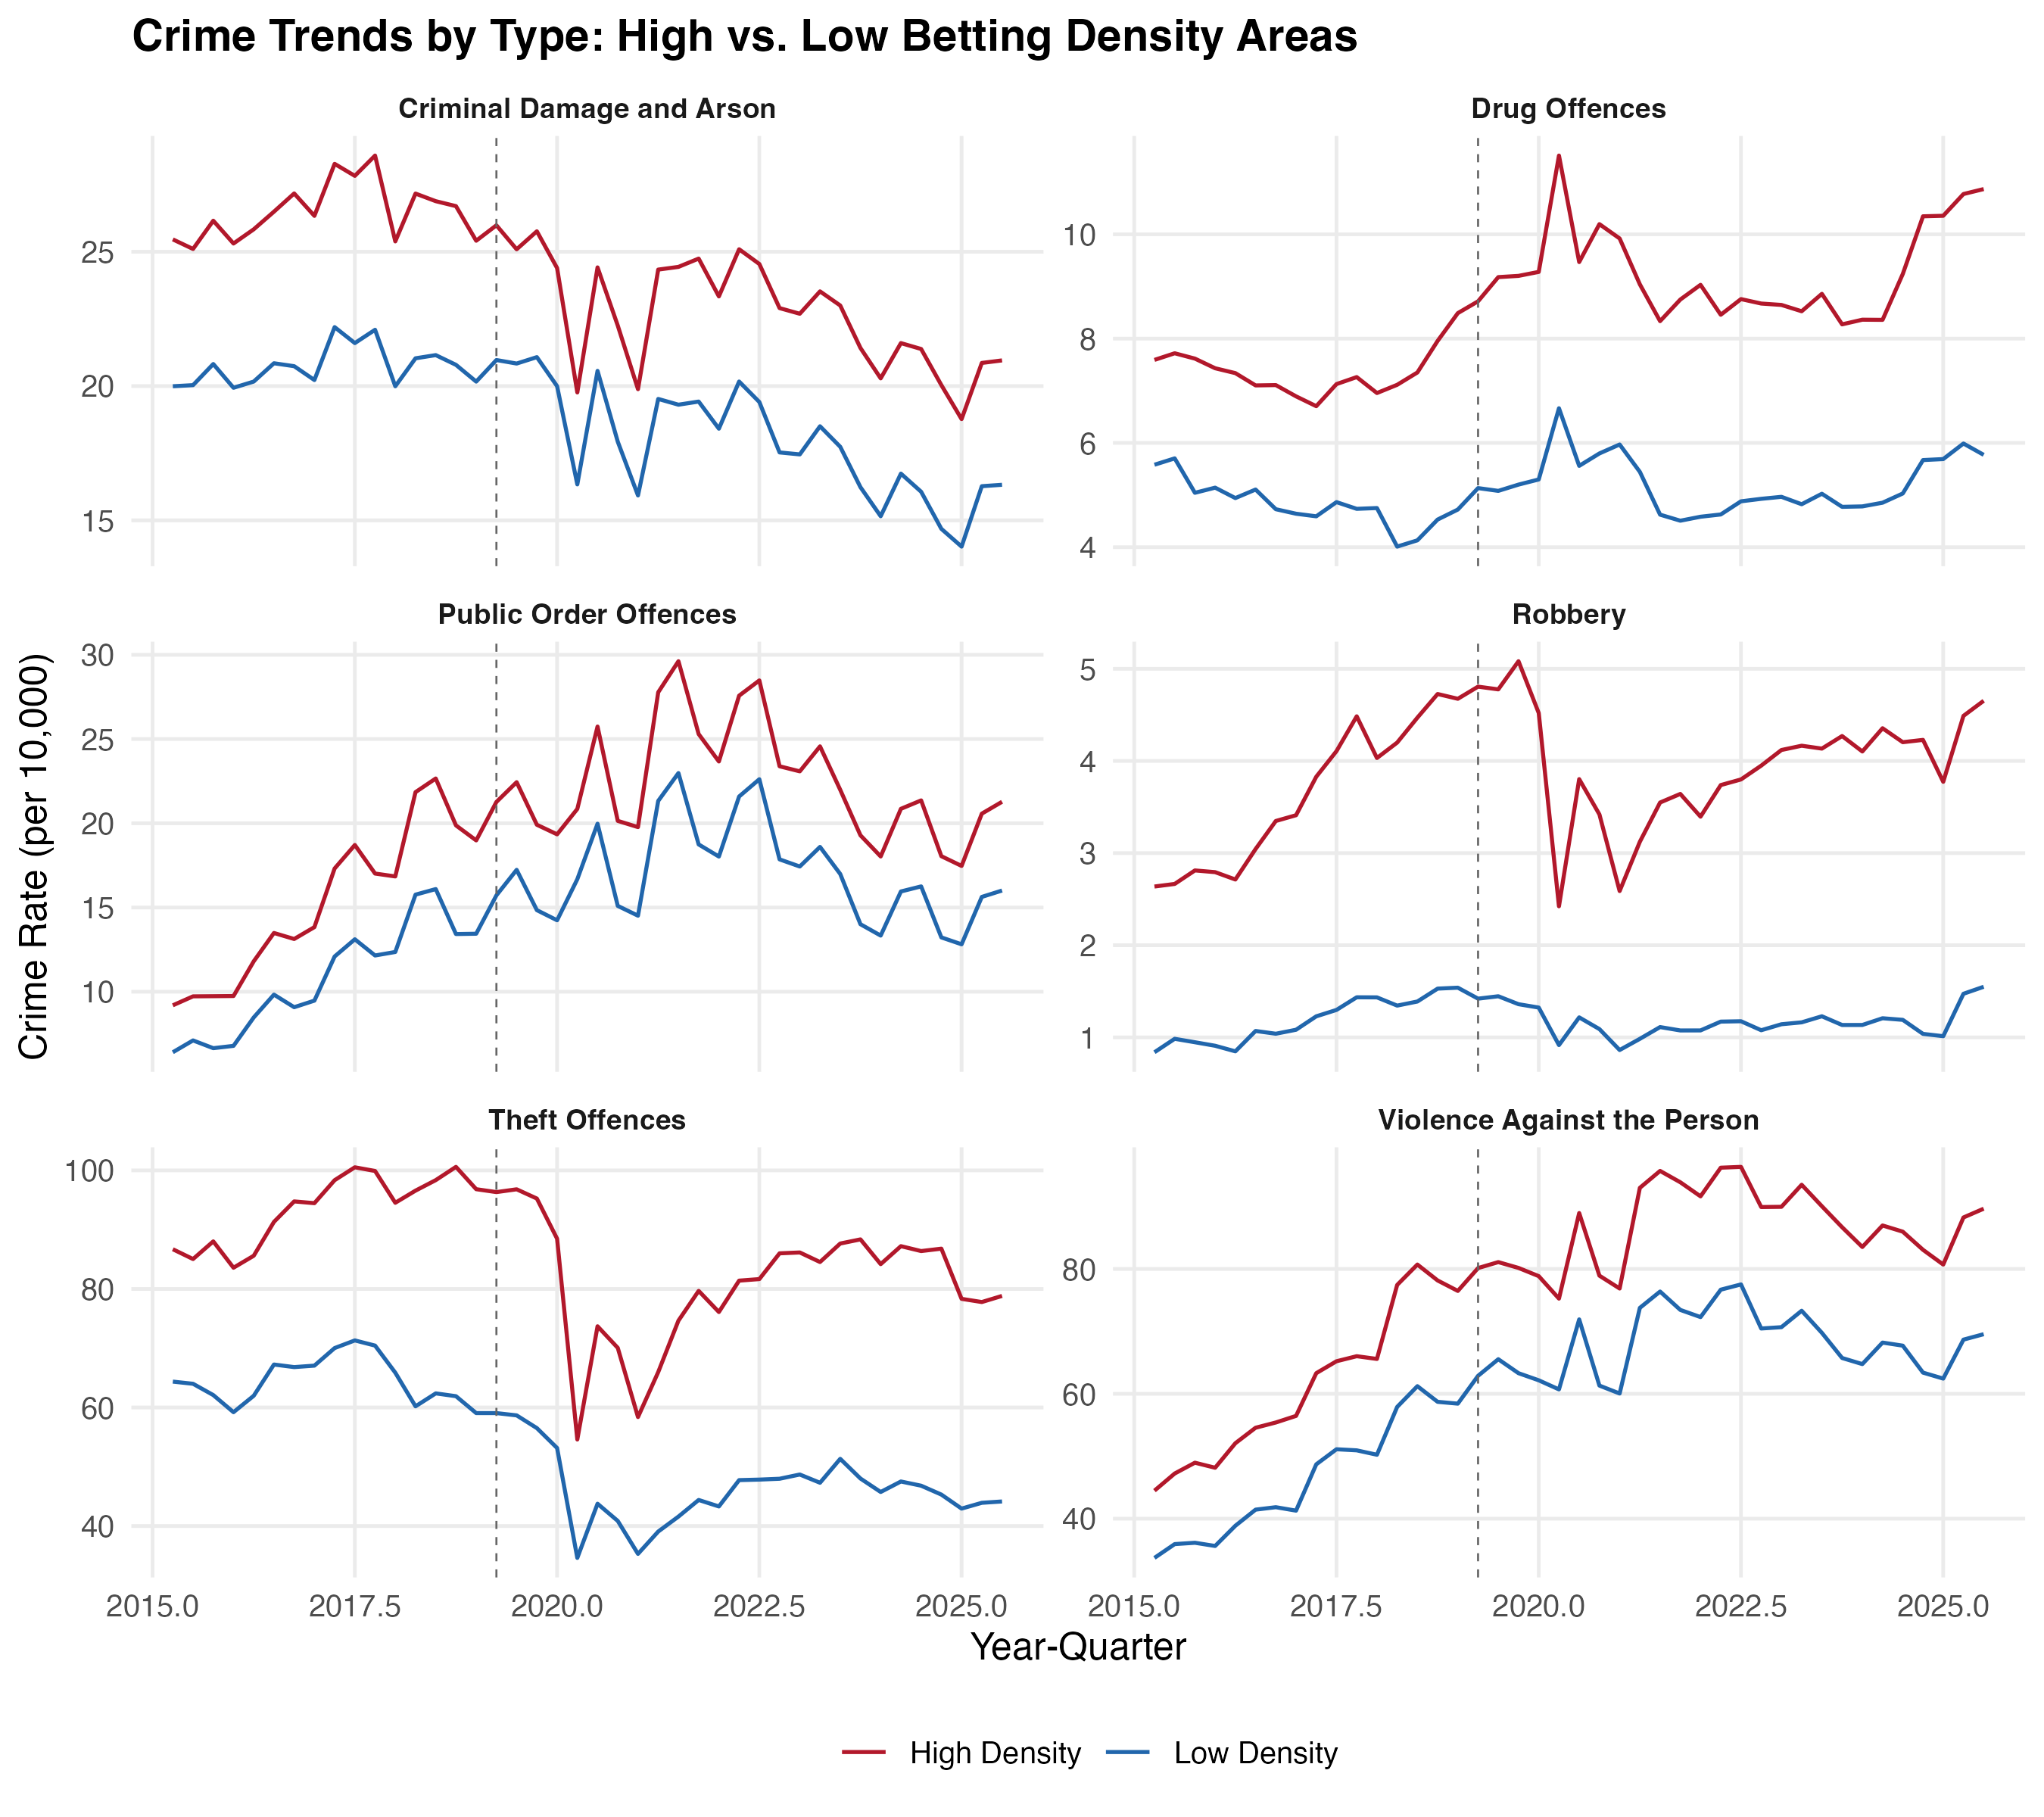
\includegraphics[width=0.9\textwidth]{figures/fig4_crime_decomposition.png}
\caption{Crime Trends by Offence Group: High vs.\ Low Density Areas}
\label{fig:decomp}
\floatfoot{\textit{Notes:} Mean crime rates per 10,000 by quarter for areas above (red) and below (blue) median betting density. Dashed line indicates policy implementation.}
\end{figure}

\section{Robustness Appendix}
\label{app:robustness}

\subsection{Distribution of Betting Density}

\begin{figure}[H]
\centering
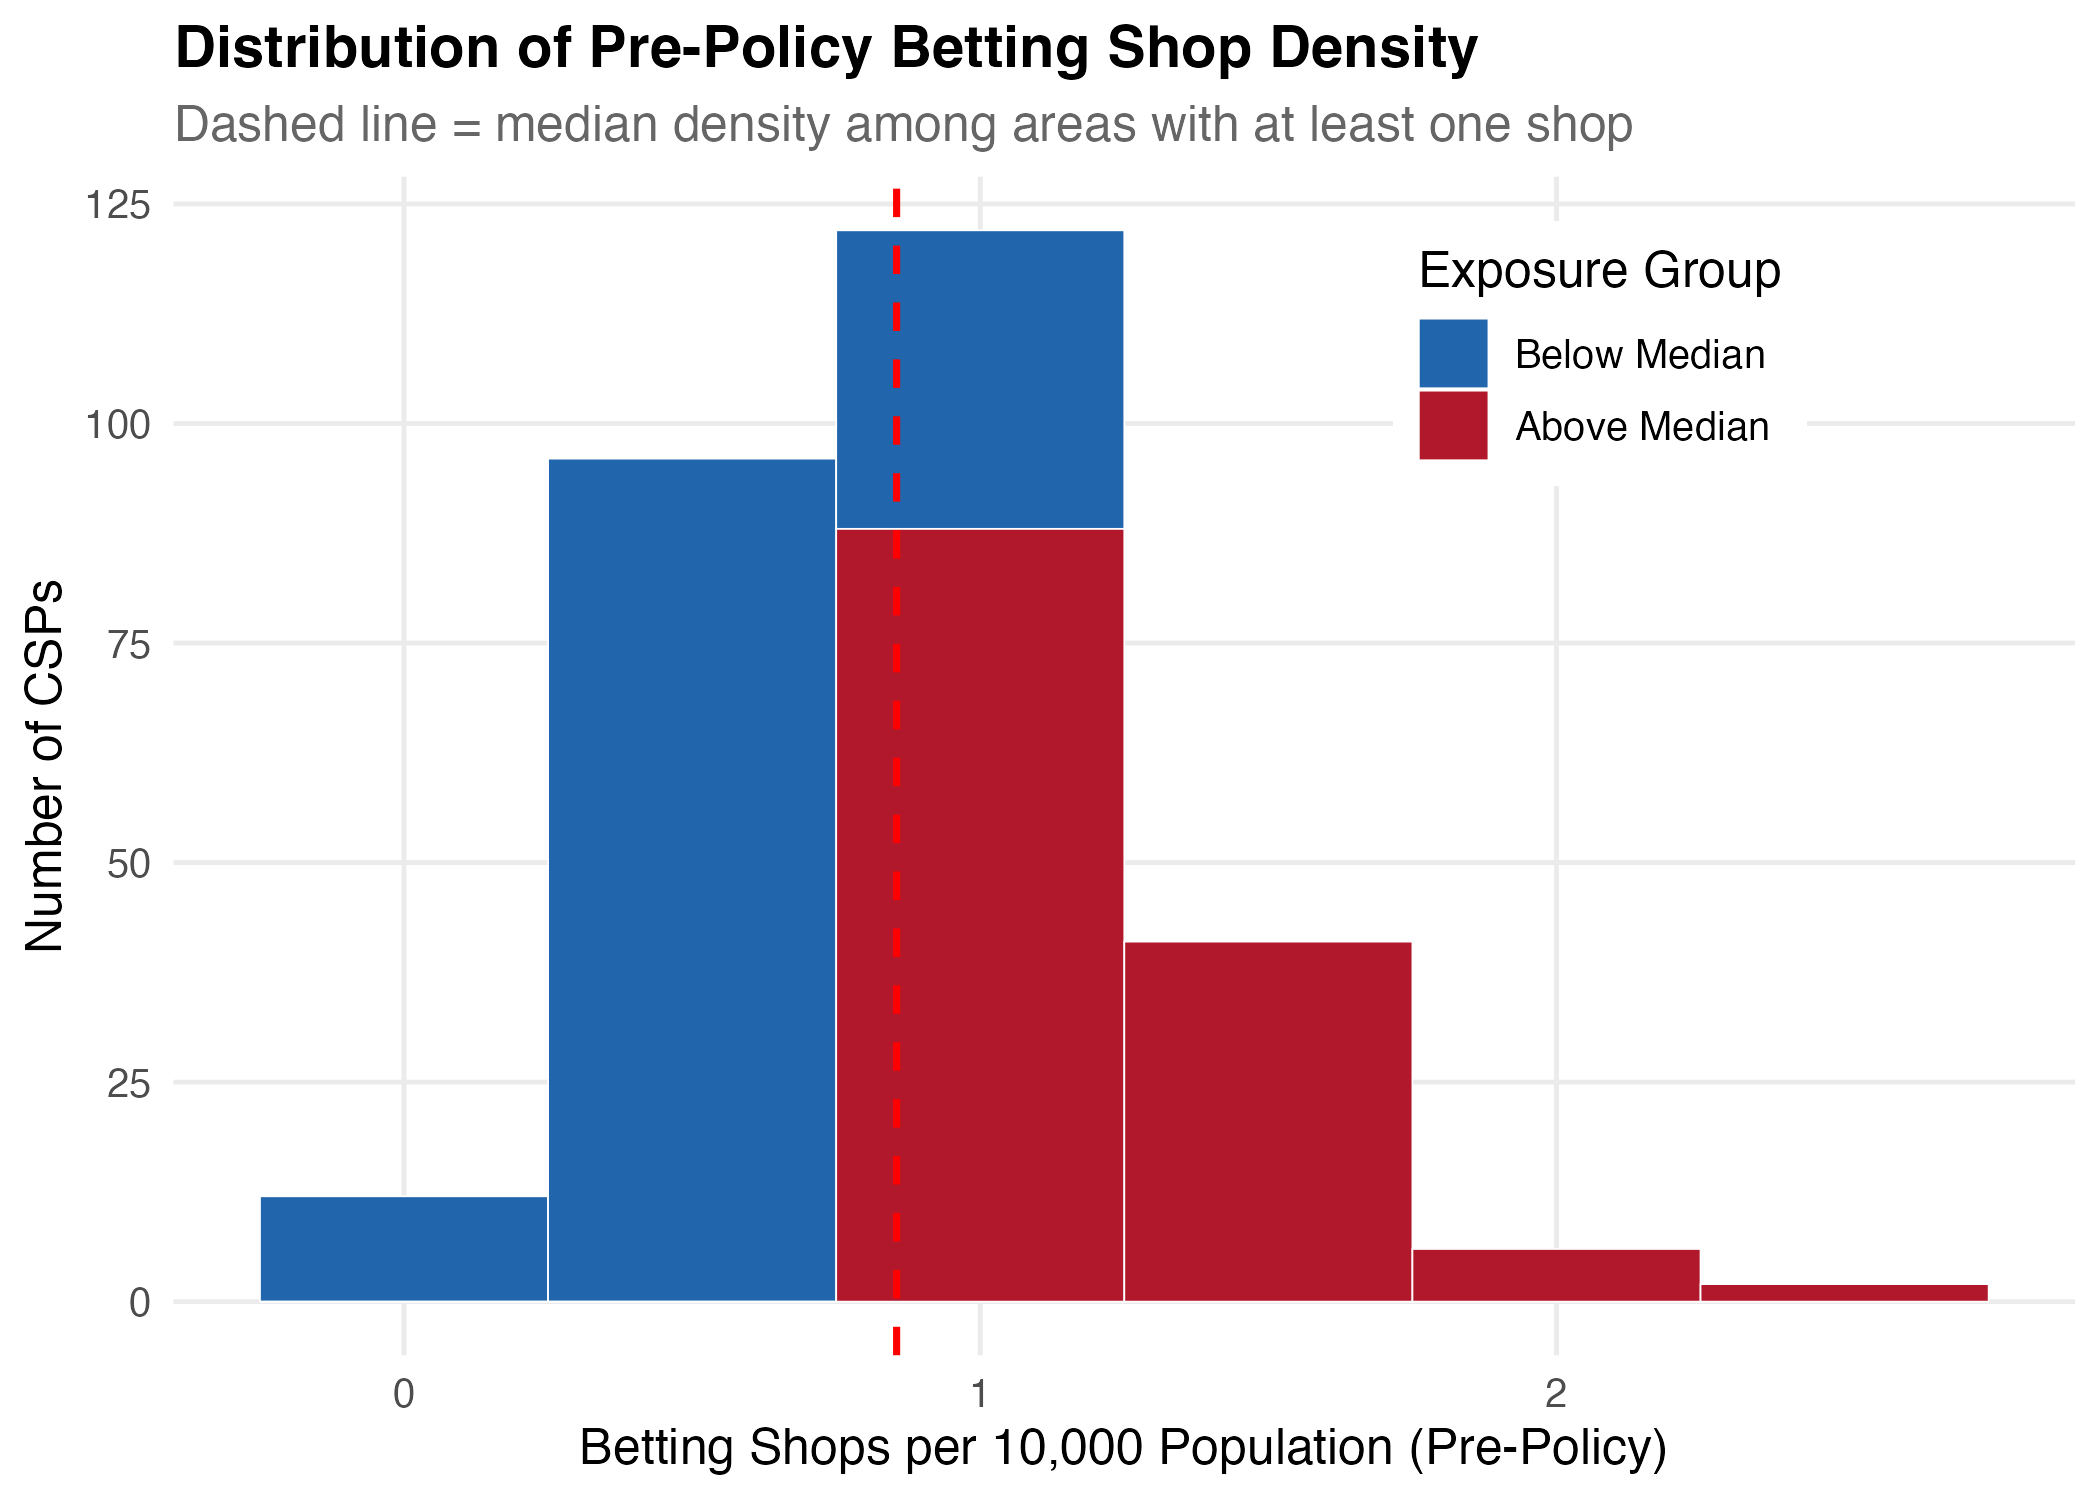
\includegraphics[width=0.8\textwidth]{figures/fig1_density_distribution.png}
\caption{Distribution of Betting Shop Density Across CSPs (Current Post-Closure Snapshot)}
\label{fig:density}
\floatfoot{\textit{Notes:} Histogram of betting shops per 10,000 population across 279 CSPs. Red/blue indicates above/below median density. Dashed line shows the median.}
\end{figure}

\subsection{Crime Trends}

\begin{figure}[H]
\centering
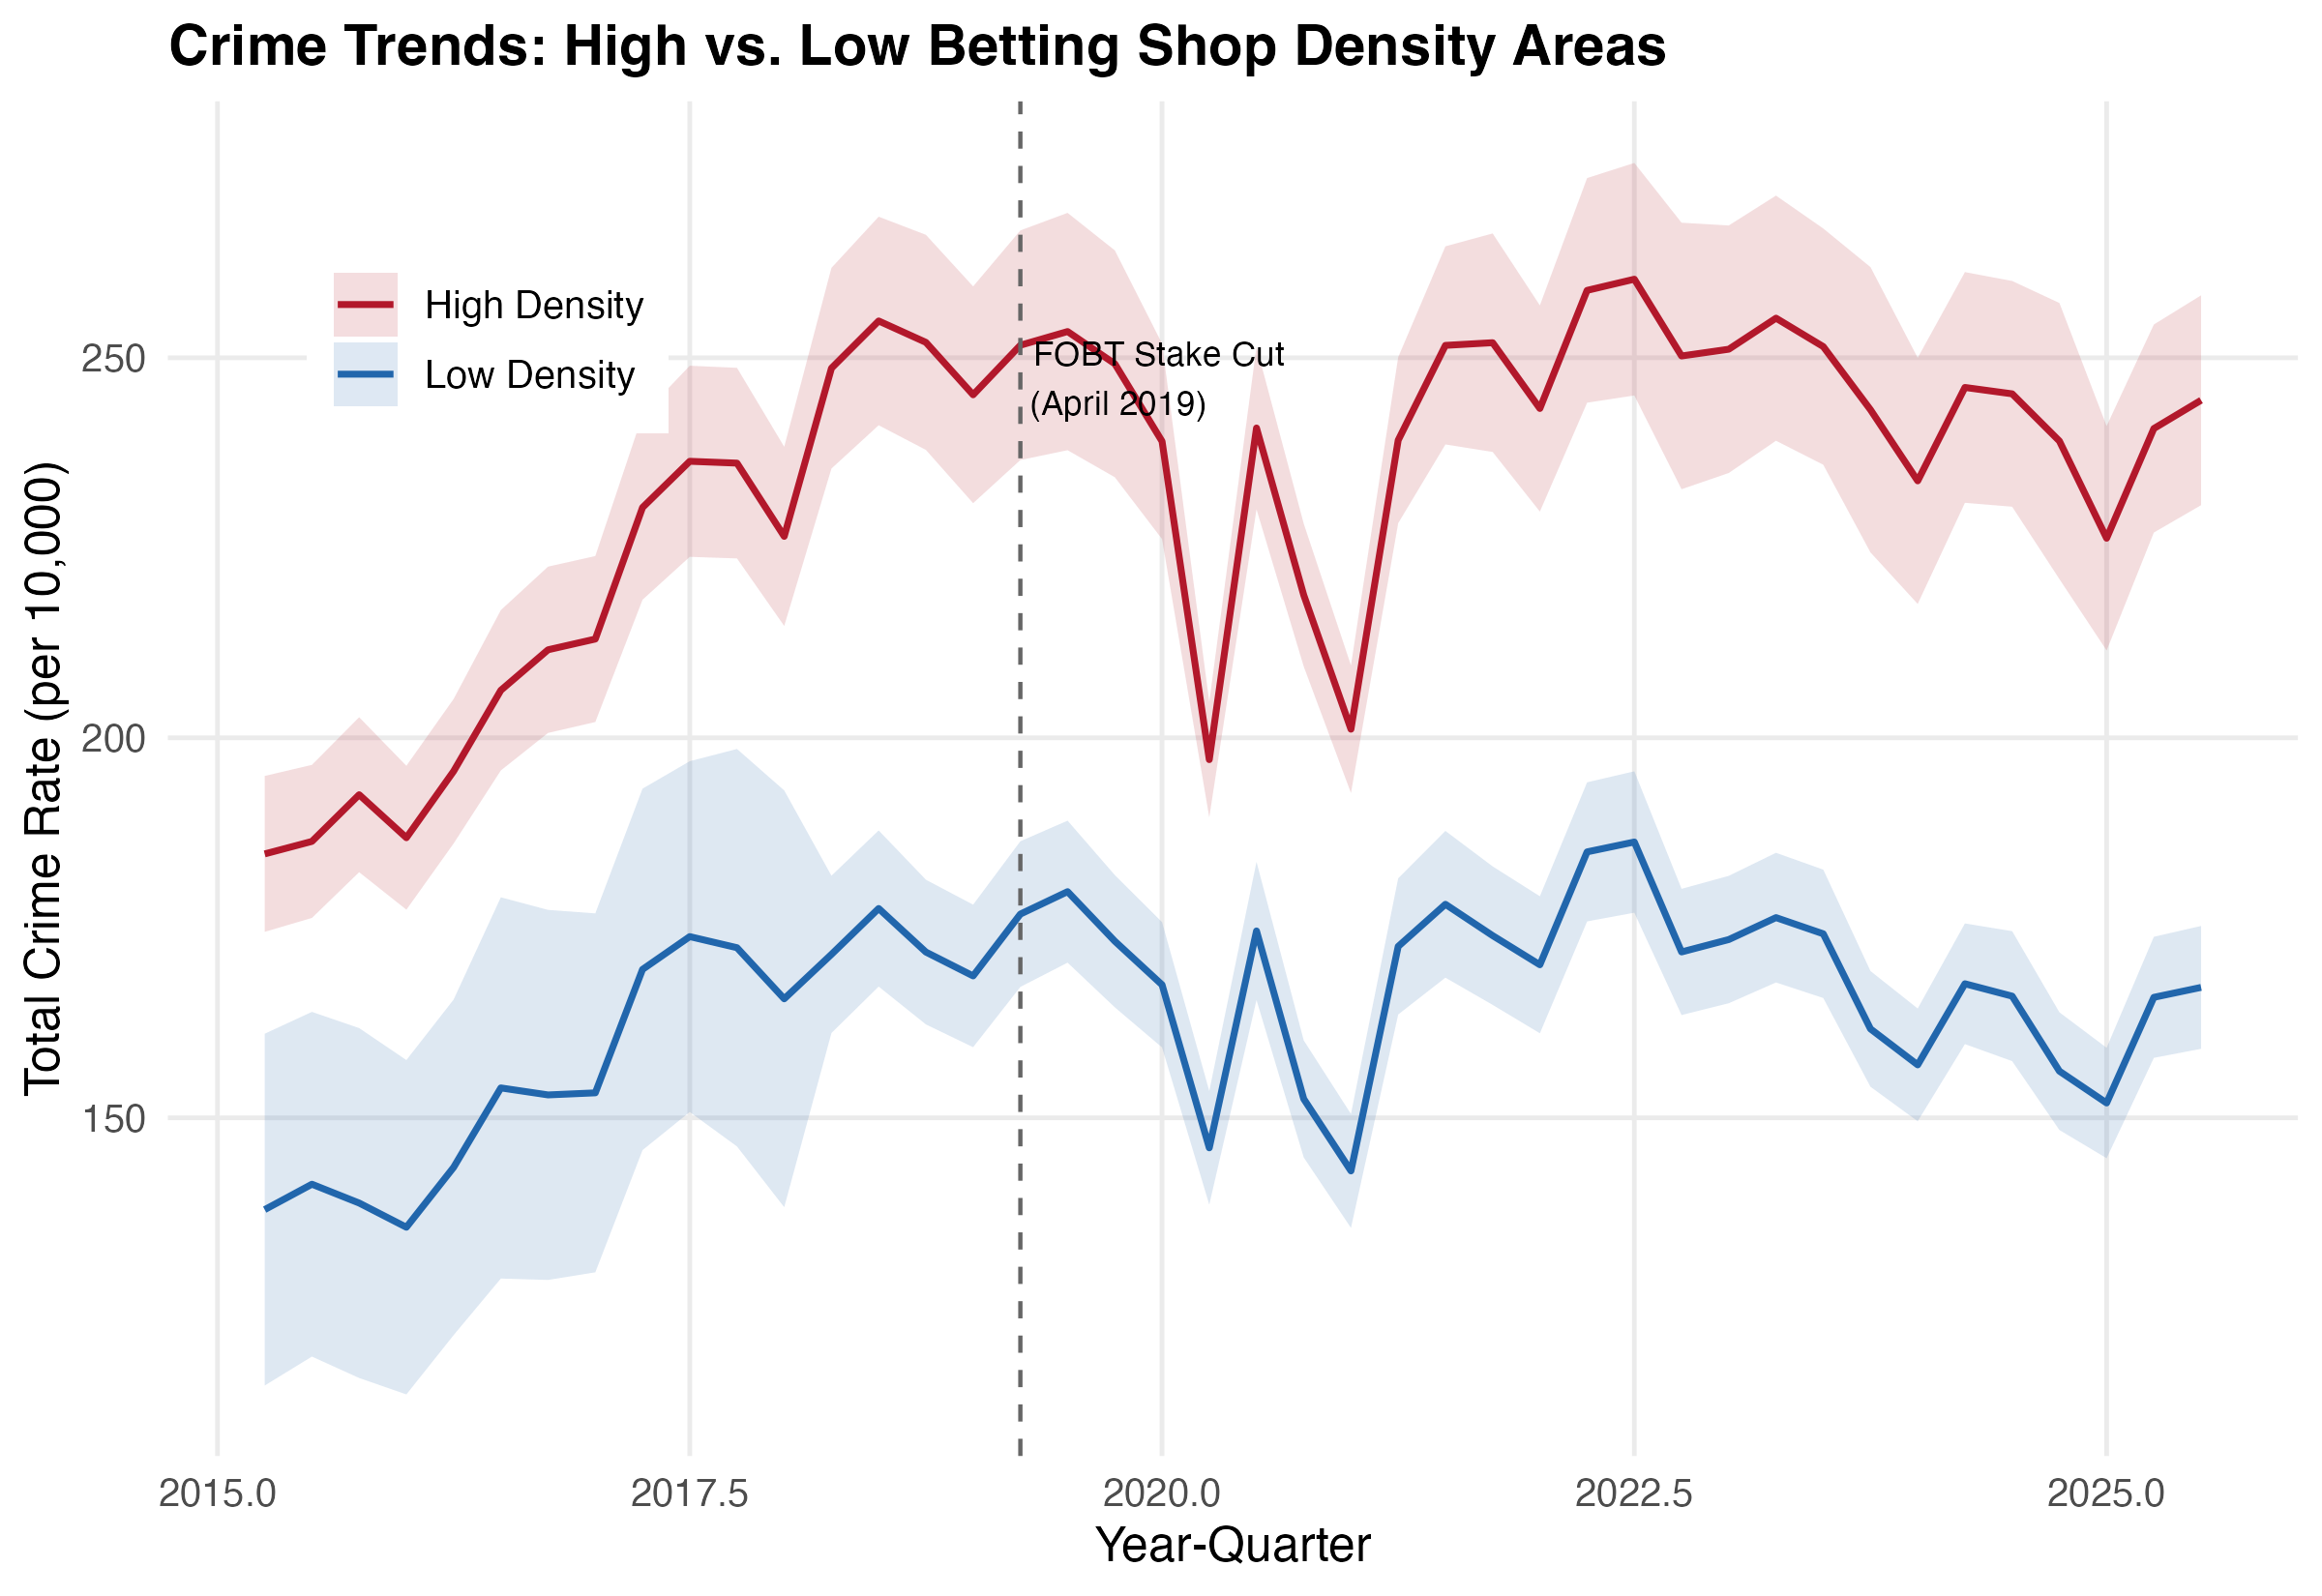
\includegraphics[width=0.85\textwidth]{figures/fig2_crime_trends.png}
\caption{Total Crime Rate Trends: High vs.\ Low Betting Density Areas}
\label{fig:trends}
\floatfoot{\textit{Notes:} Mean total crime rate per 10,000 with 95\% confidence bands. High density (red) = above median. Dashed line indicates policy implementation.}
\end{figure}


\subsection{Dose-Response}

\begin{figure}[H]
\centering
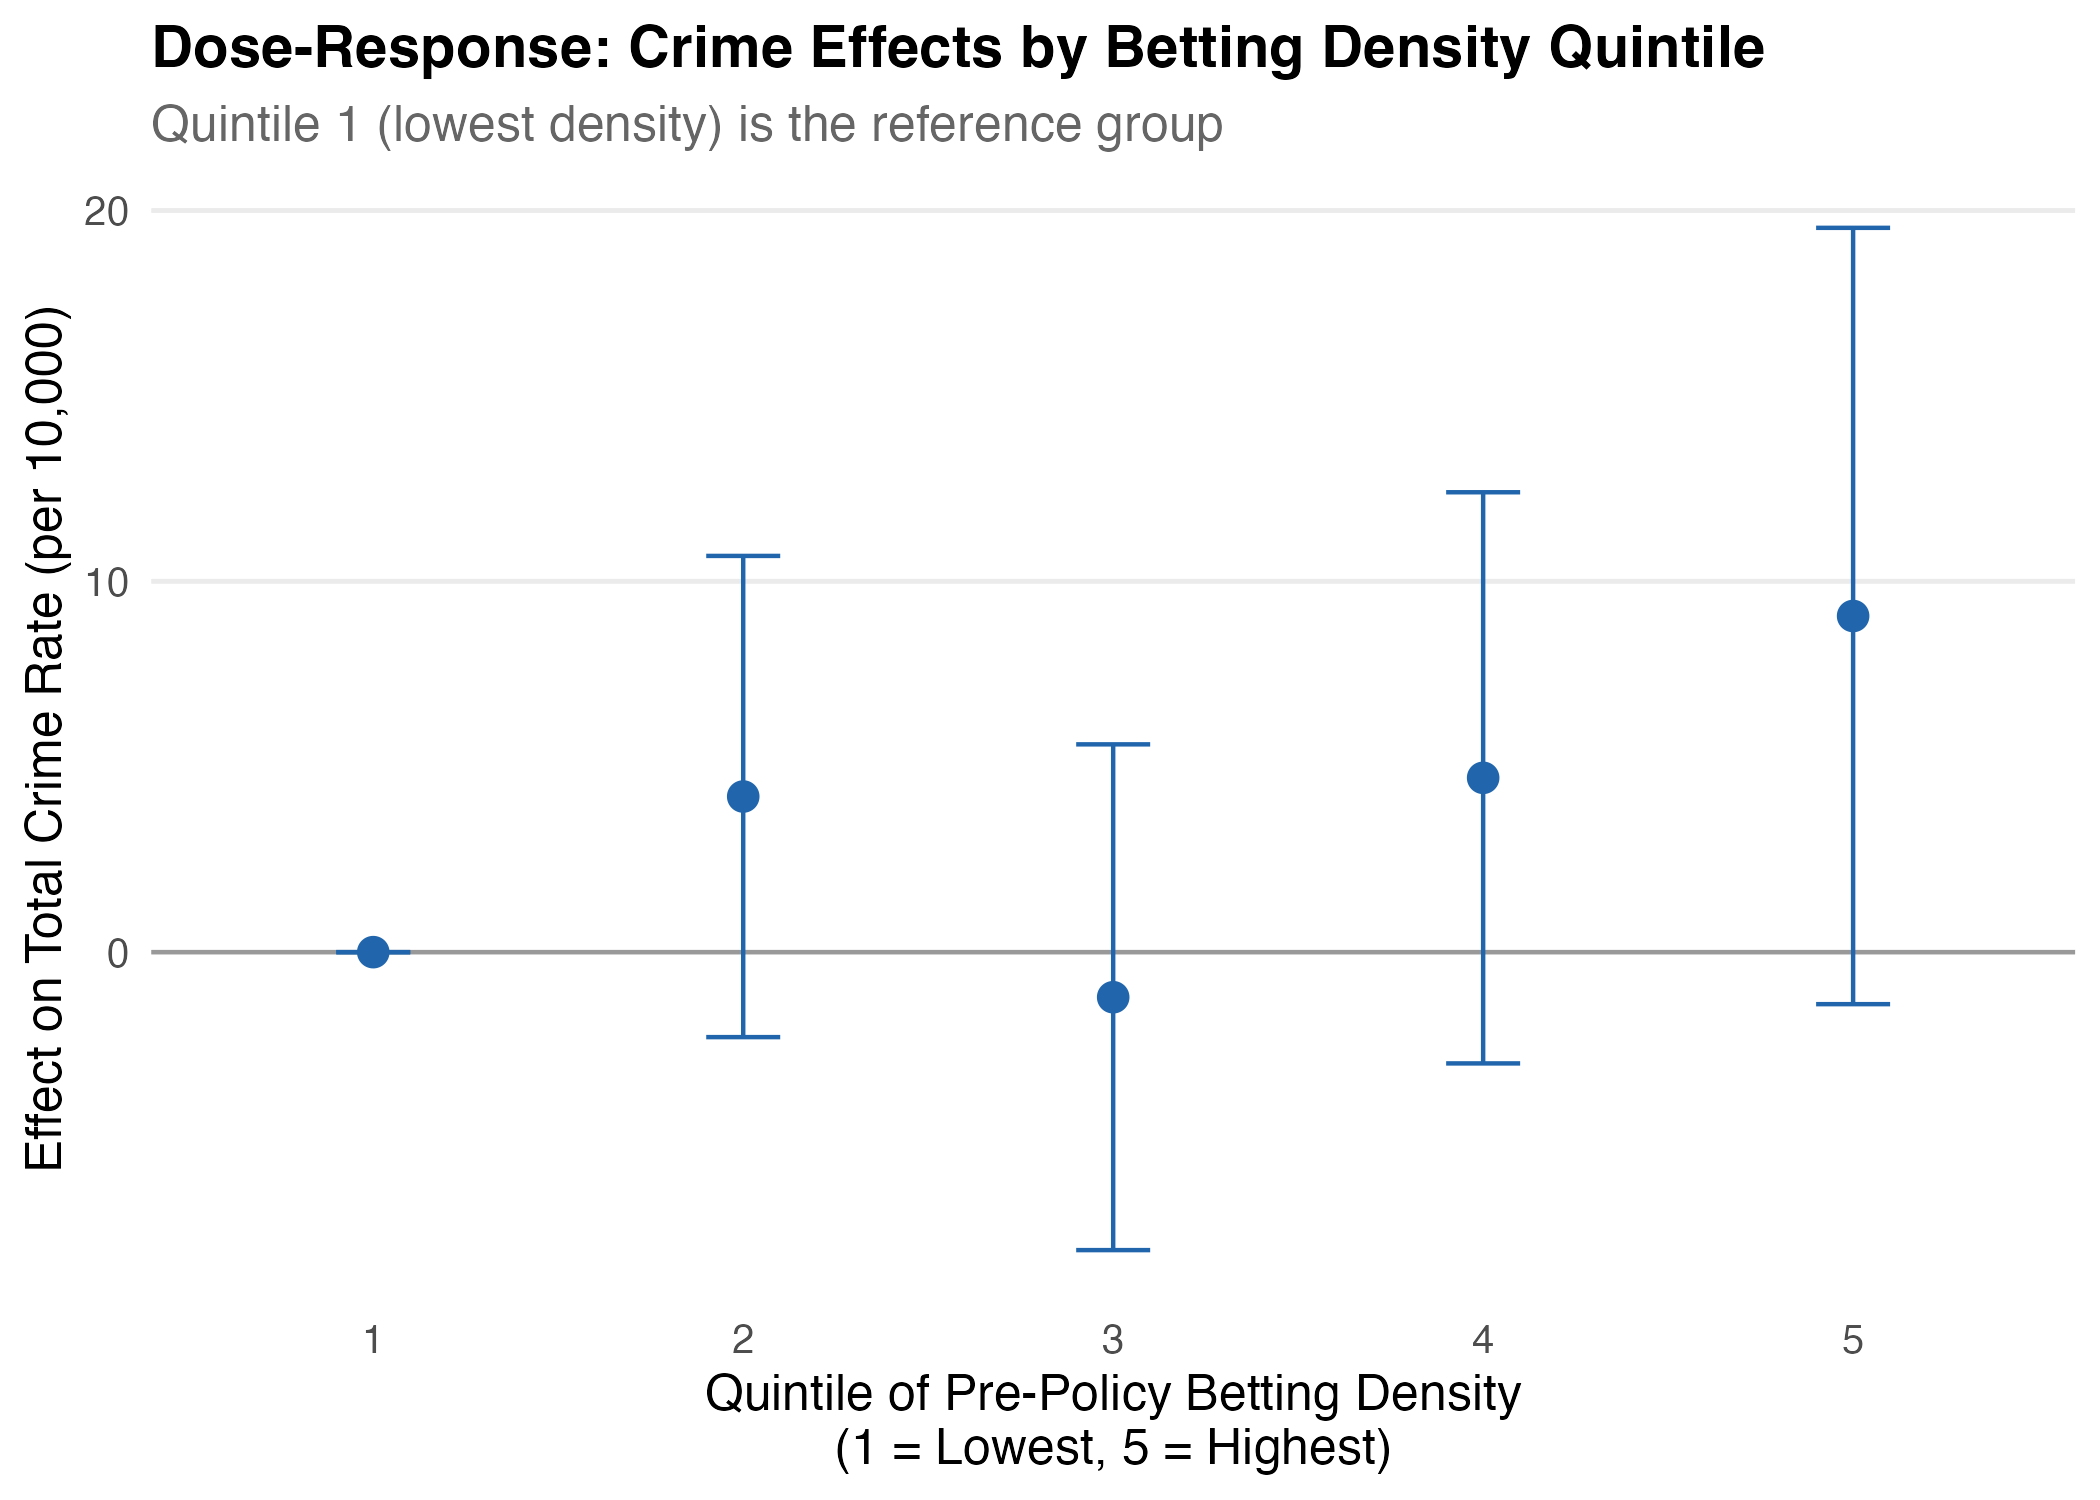
\includegraphics[width=0.75\textwidth]{figures/fig5_dose_response.png}
\caption{Dose-Response: Crime Effects by Quintile of Betting Density}
\label{fig:dose}
\floatfoot{\textit{Notes:} Point estimates and 95\% confidence intervals for the interaction of density quintile $\times$ Post, relative to quintile 1 (lowest density). Standard errors clustered at CSP level.}
\end{figure}

\section{Heterogeneity Appendix}

No additional heterogeneity analyses beyond those presented in the main text.

\section{Additional Figures and Tables}

All exhibits are presented in the main text and appendix sections above.

\end{document}
